
\begin{section}{Simulation Results}
\label{sec:simulation}

% Need to label states of the state vector in the modeling section [x y v \theta]

The case study investigated in this paper is with a ground vehicle experiencing the effects of sensor and process noise, dynamical changes, while also succumbing to wind disturbances and sensor attacks. The vehicle will be traveling along a pre-planned trajectory with assumed to be known obstacles throughout the environment. We consider a ground vehicle starting at an initial position $\bm{p}(0)=\begin{bmatrix} 22,10 \end{bmatrix}^T$ facing the positive $x$ direction with zero velocity. The objective for the vehicle is to reach a goal point while following a desired trajectory with obstacles of varying distances from the path. It is assumed the maximum velocity of the vehicle is 3.0m/s and the desired reference velocity it wants to maintain is 2.5m/s. For simulations...




\begin{figure*}[b!th]
%\begin{figure*}[th!]
\begin{tabular}{ccc}

\subfigure[\label{fig:low_noise} ]{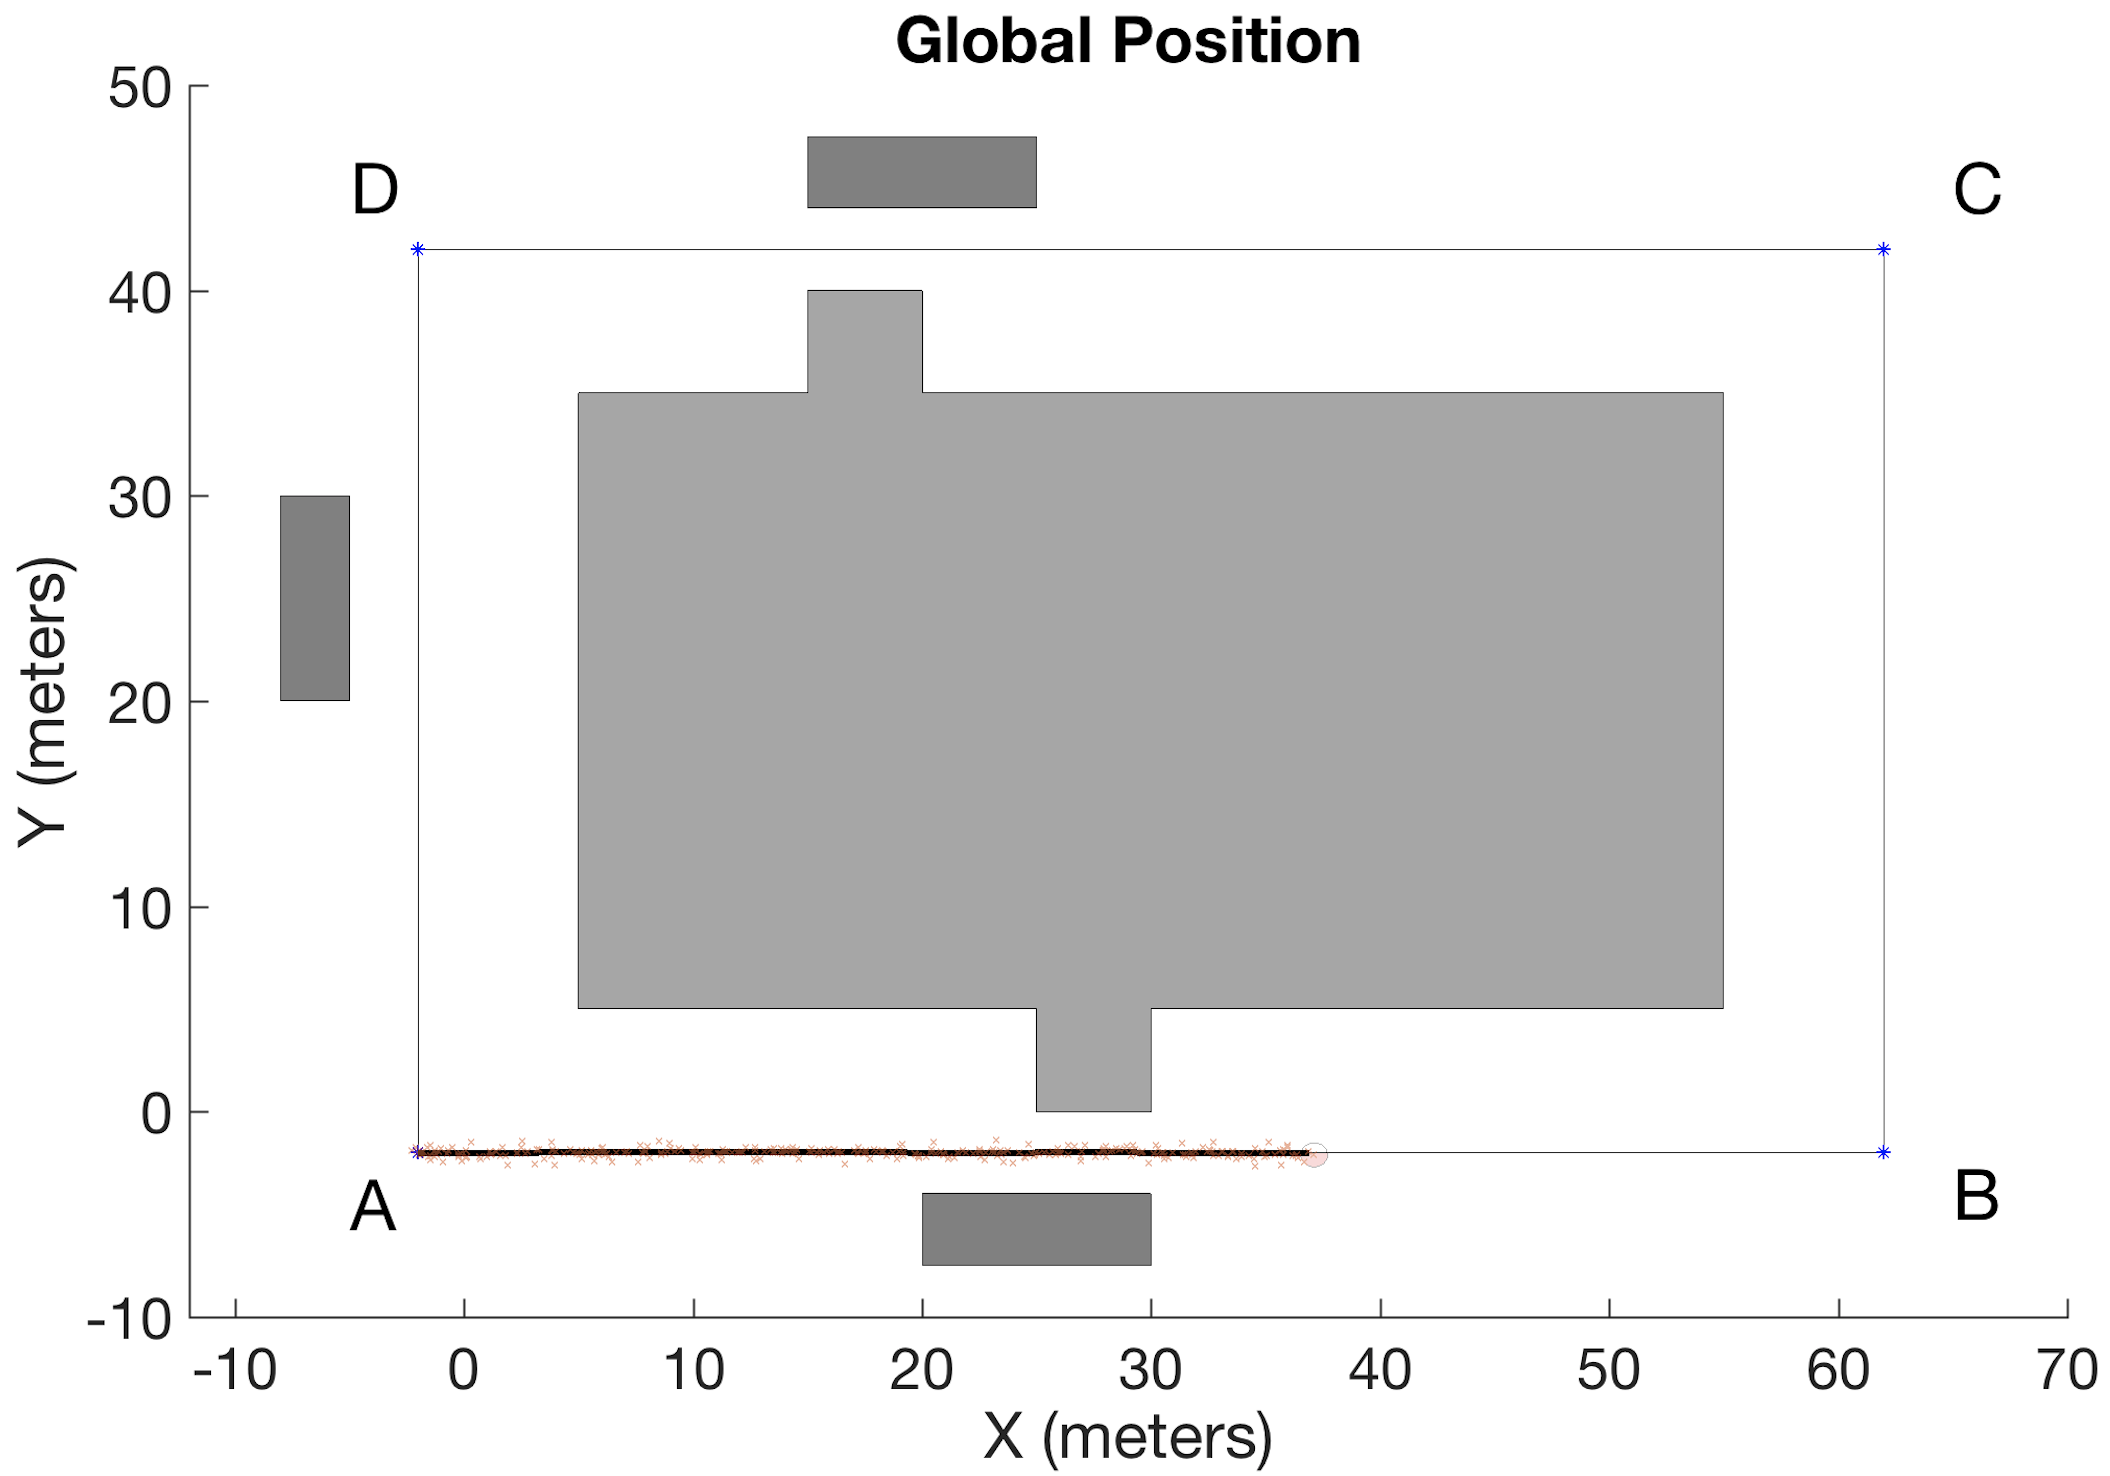
\includegraphics[width = 0.3\textwidth]{Figures/Motion1.png}} &	
\subfigure[\label{fig:low_noise2} ]{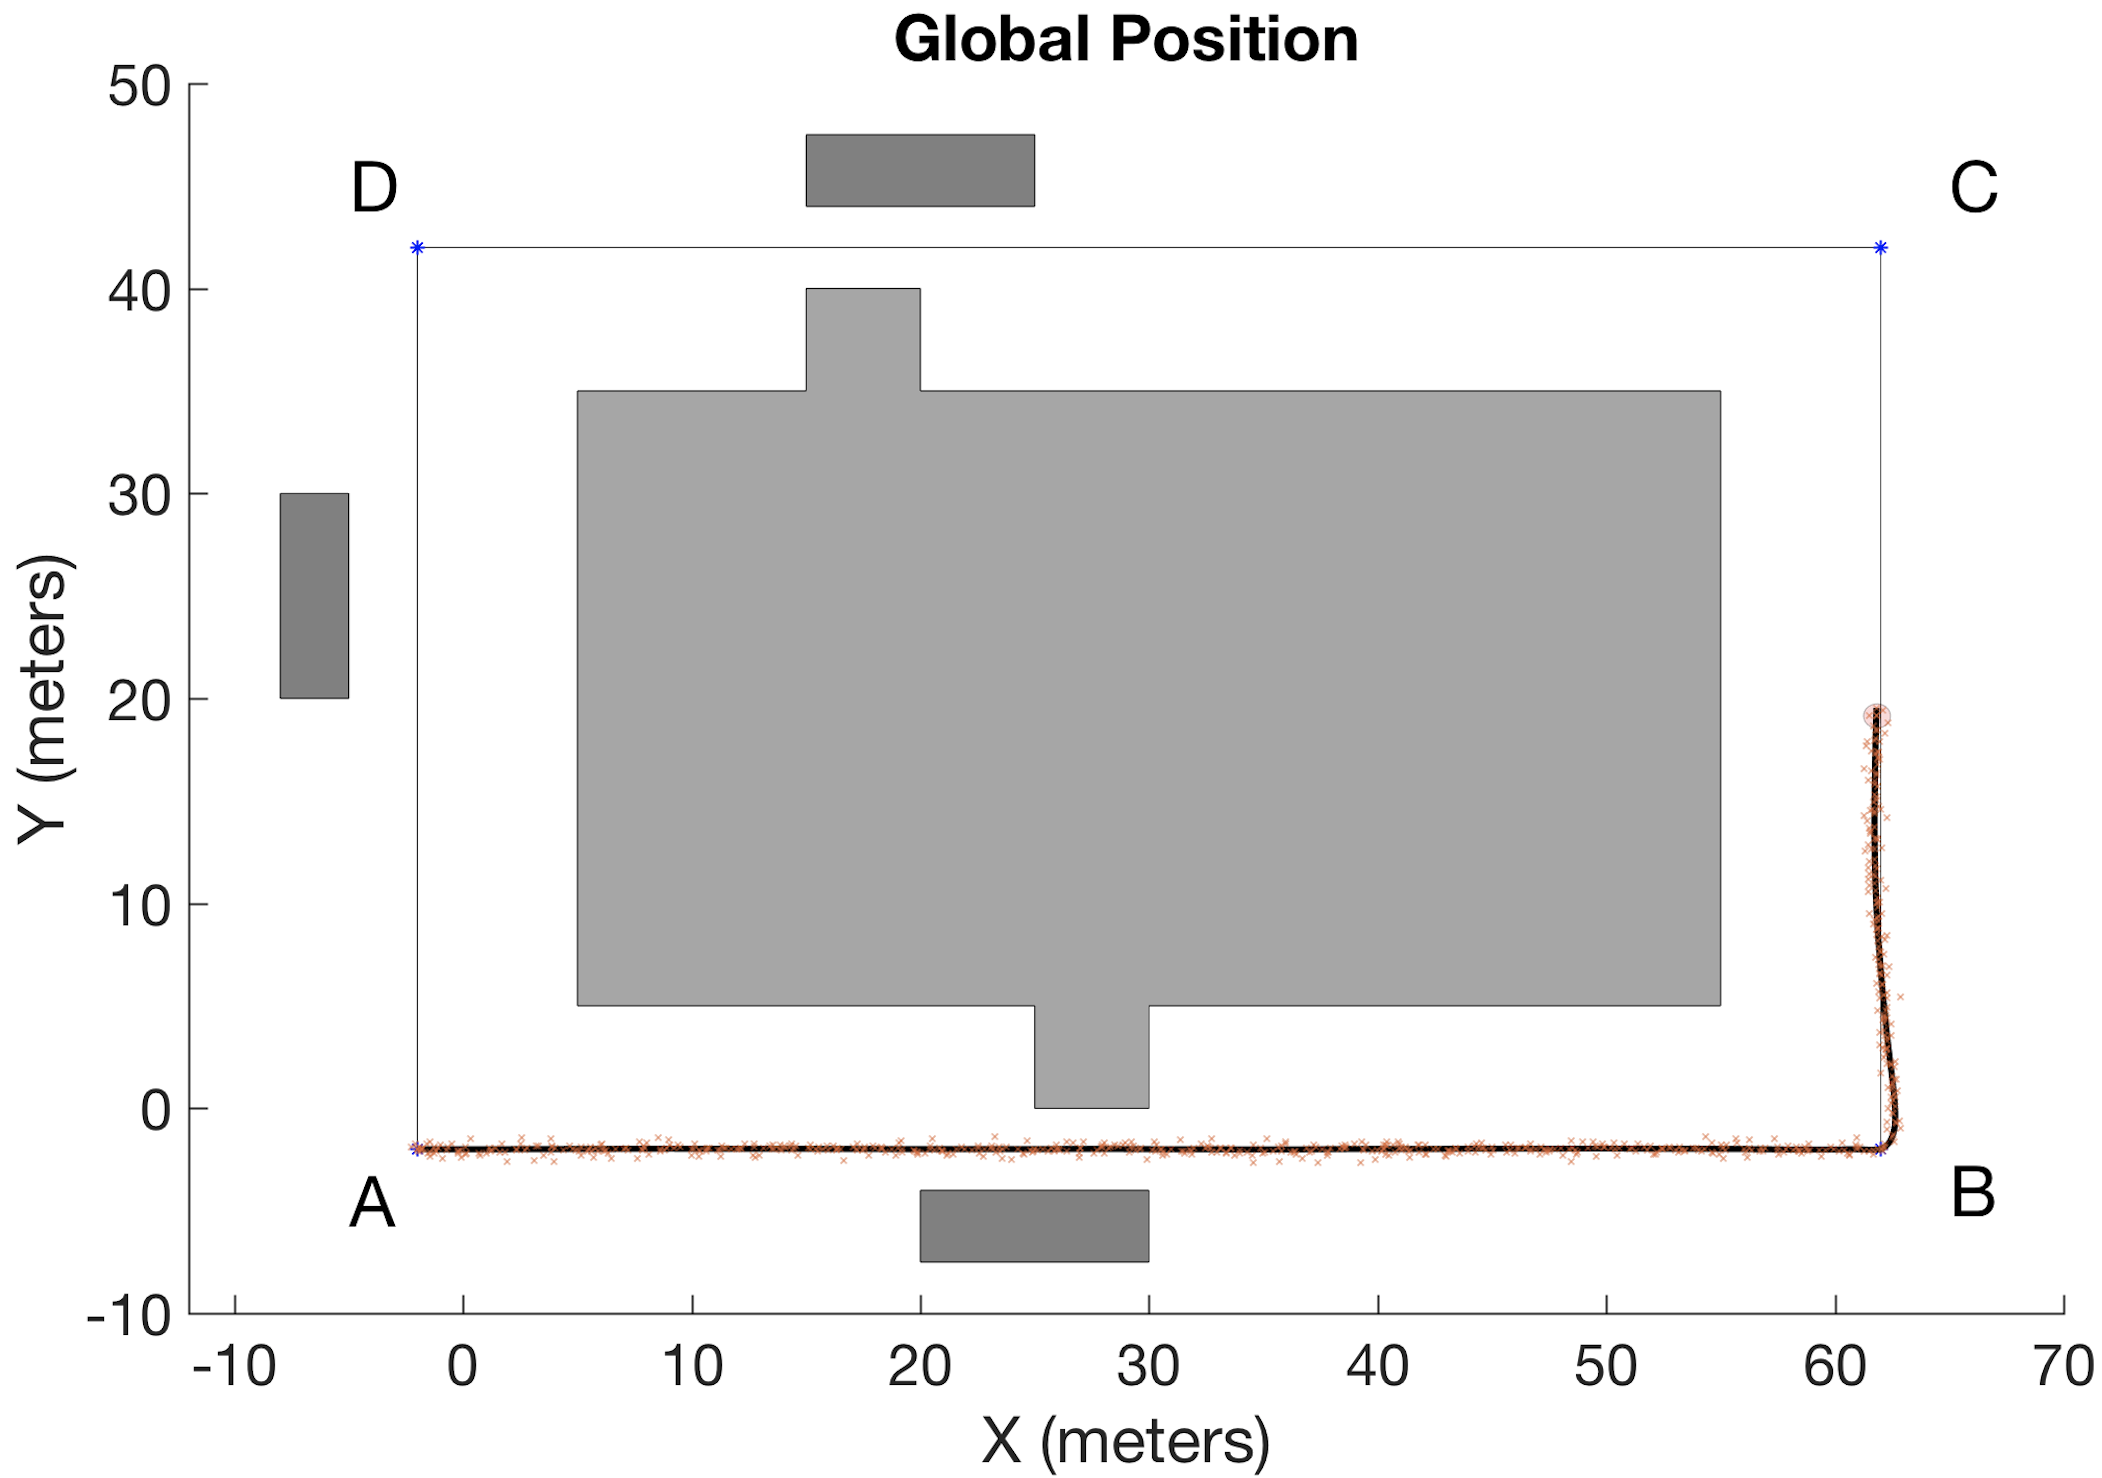
\includegraphics[width = 0.3\textwidth]{Figures/Motion2.png}} &
\subfigure[\label{fig:at_attack} ]{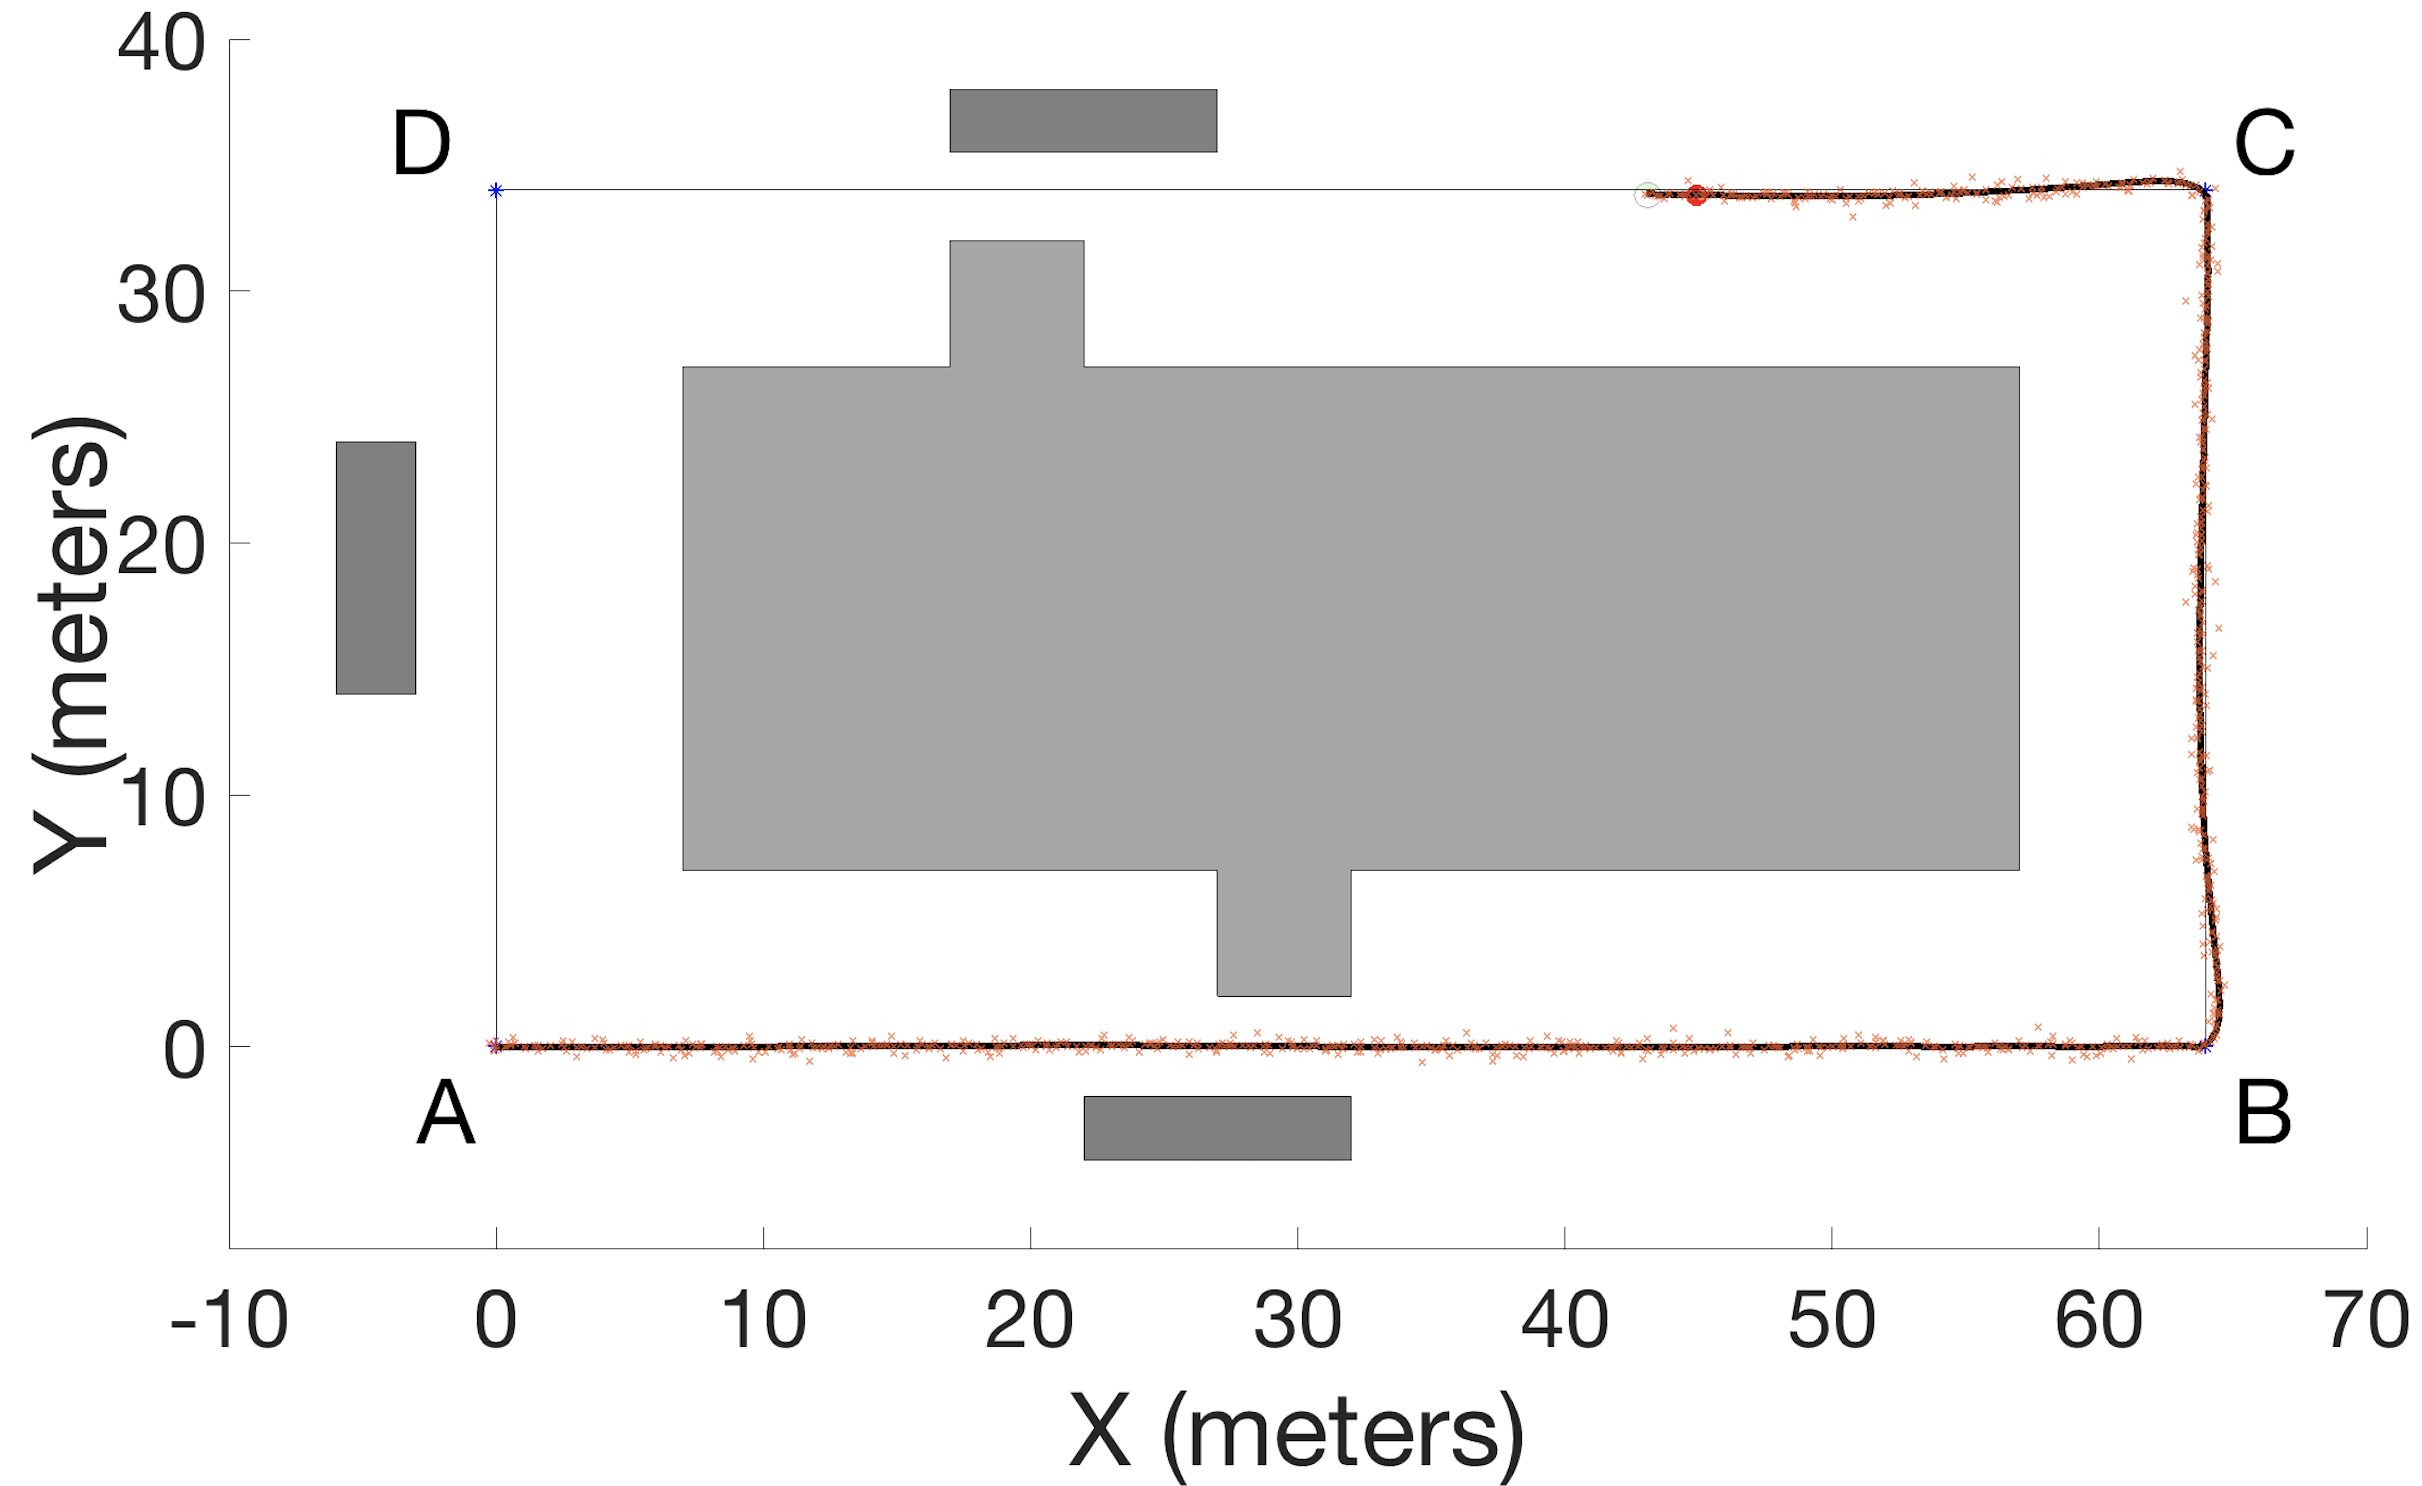
\includegraphics[width = 0.3\textwidth]{Figures/Motion3.png}}
\end{tabular} \\
\begin{tabular}{ccc}
\subfigure[\label{fig:after_detection} ]{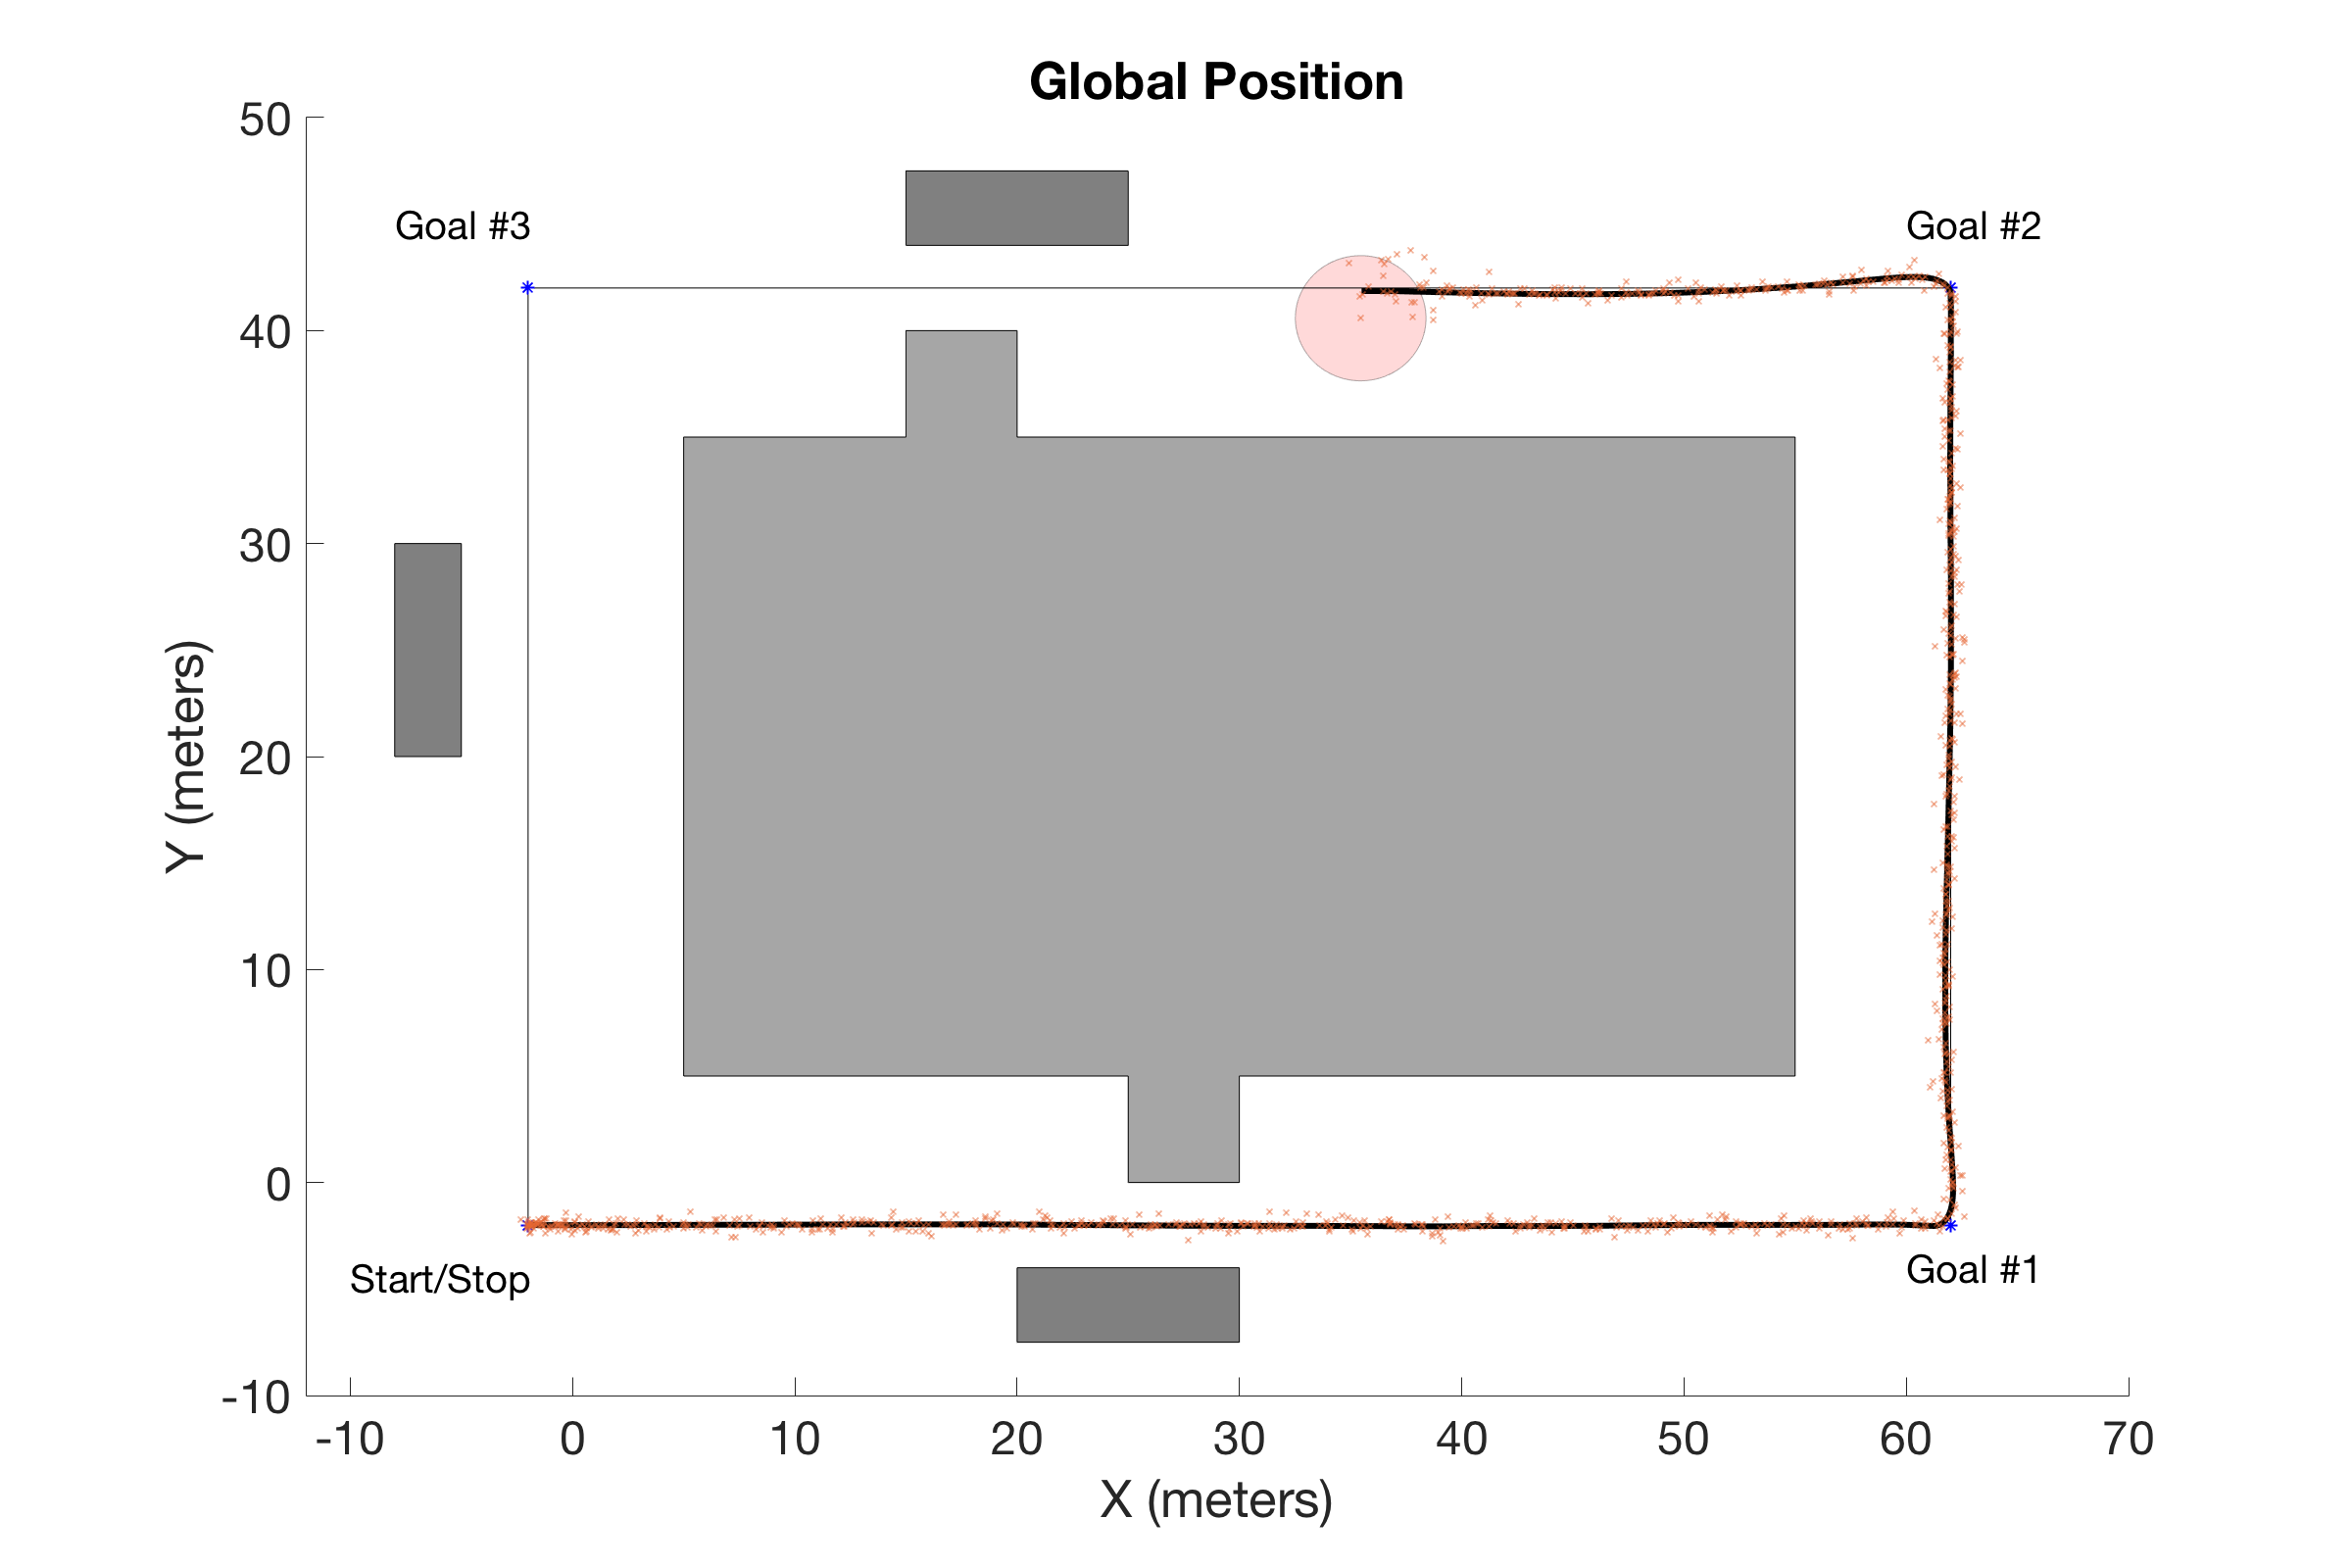
\includegraphics[width = 0.3\textwidth]{Figures/Motion4.png}} &
\subfigure[\label{fig:adapt_region} ]{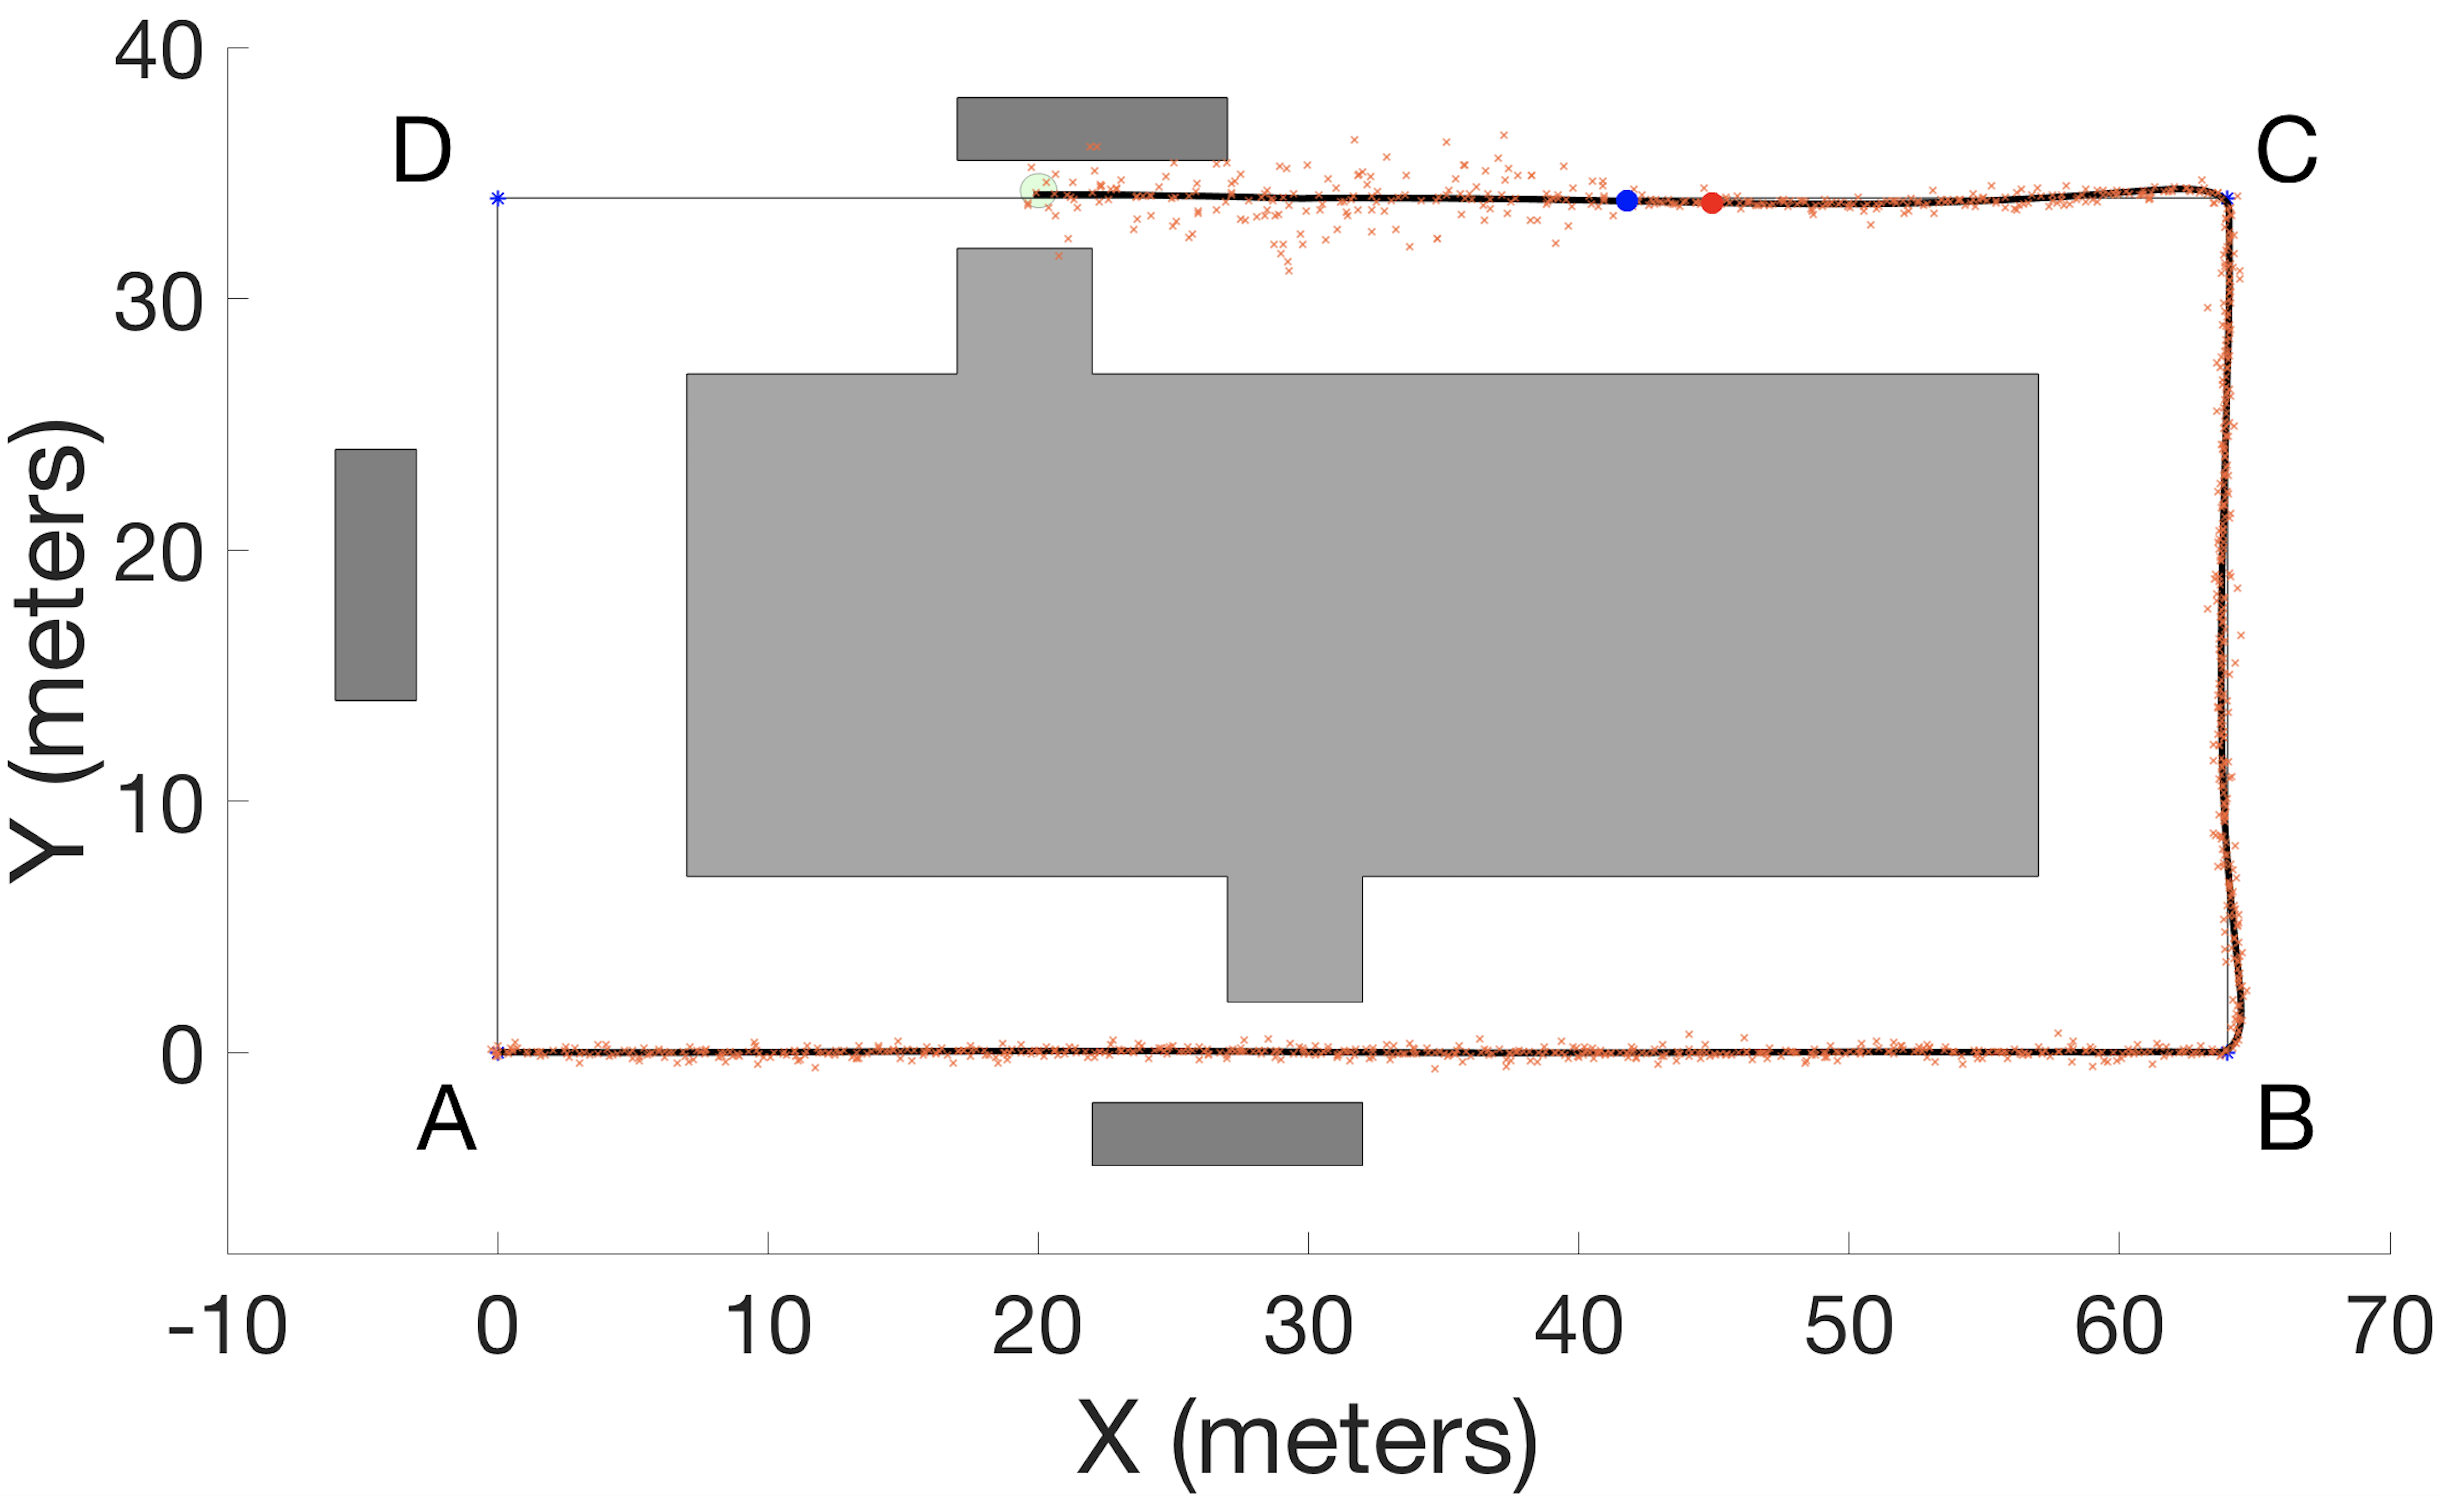
\includegraphics[width = 0.3\textwidth]{Figures/Motion5.png}} & 
\subfigure[\label{fig:continue_motion} ]{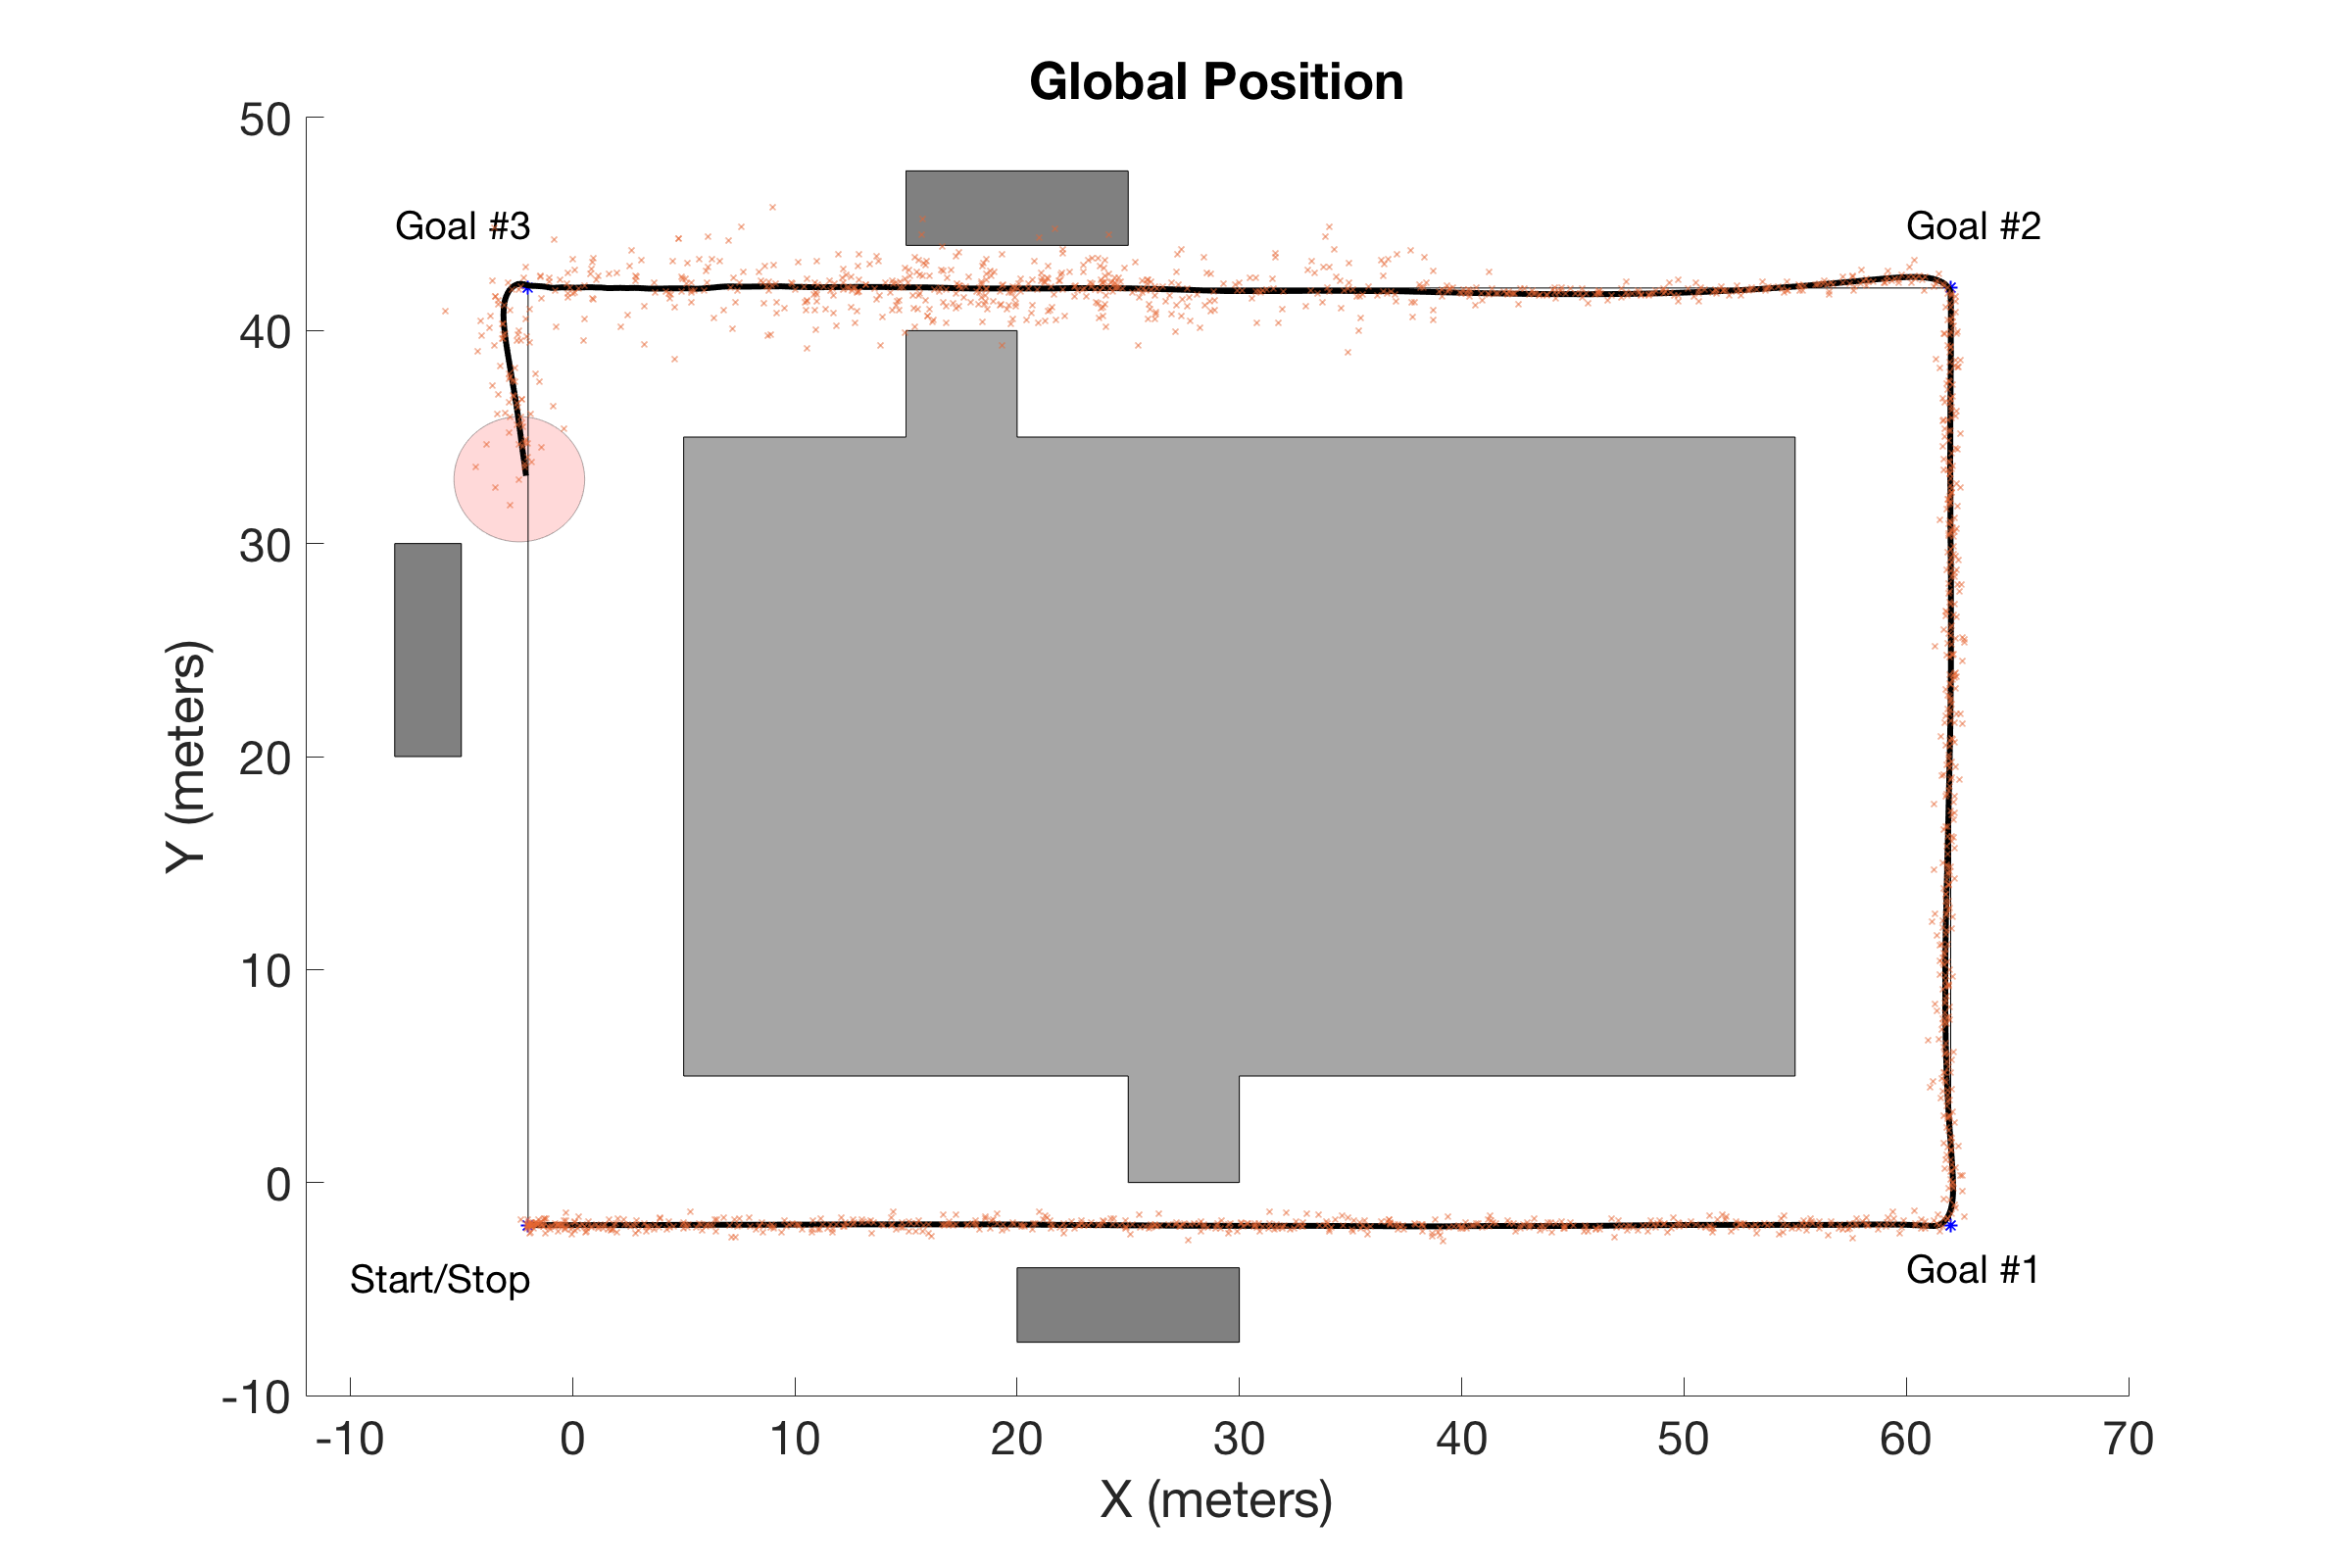
\includegraphics[width = 0.3\textwidth]{Figures/Motion6.png}}

\end{tabular}
\caption{A comparison in time of a vehicle navigating through an obstacle filled environment. In (a), the sensors at this time are uncompromised, with low uncertainty,..... undecided if I should explain all the figures here or just do it in the text... }

\end{figure*}

In Figure \ref{fig:low_noise}, the vehicle moving along the trajectory with no compromised sensors and far from obstacles. The confidence region is, in general, small because the best available sensors with low amount of noise are available . Velocity is unaltered due to the obstacles being well outside the uncertainty boundaries.

While all sensors are uncompromised, Figure \ref{fig:low_noise2} shows a region where the vehicle is undergoing dynamical changes. The confidence region remains unchanged due to the full uncompromised set of sensors. The adaptive controller is maintaining a reference velocity, even while system dynamics are changing.

Figure \ref{fig:at_attack} shows vehicle position at the starting time of the ramped sensor attack. The amplitude of the attack is still well within the sensor noise bounds, detection does not occur.


Detection of the spoofed sensor is demonstrated in Figure \ref{fig:after_detection}. The spoofed sensor has been removed from the system, leaving a smaller set of available sensors with higher uncertainty. The confidence region grows in size due to the changes in uncertainty. Obstacles are still well outside of the bounds, allowing the vehicle to continue navigating at its desired velocity.

Figure \ref{fig:adapt_region} shows the confidence region shrinking in size when the vehicle navigates near obstacles of closer distances. More data points are used to improve this estimation, while the velocity is reduced to lessen uncertainty while moving.

Once the vehicle is past the obstacles that are at close distances, shown in Figure \ref{fig:continue_motion}, the vehicle is able to move freely again at its desired velocity. The confidence region remains at a much larger radius due to the smaller set of available sensors.



\begin{figure}
\vspace{1pt}
\centering
\begin{tabular}{cc}

\subfigure[\label{fig:vel_G1and2} ]{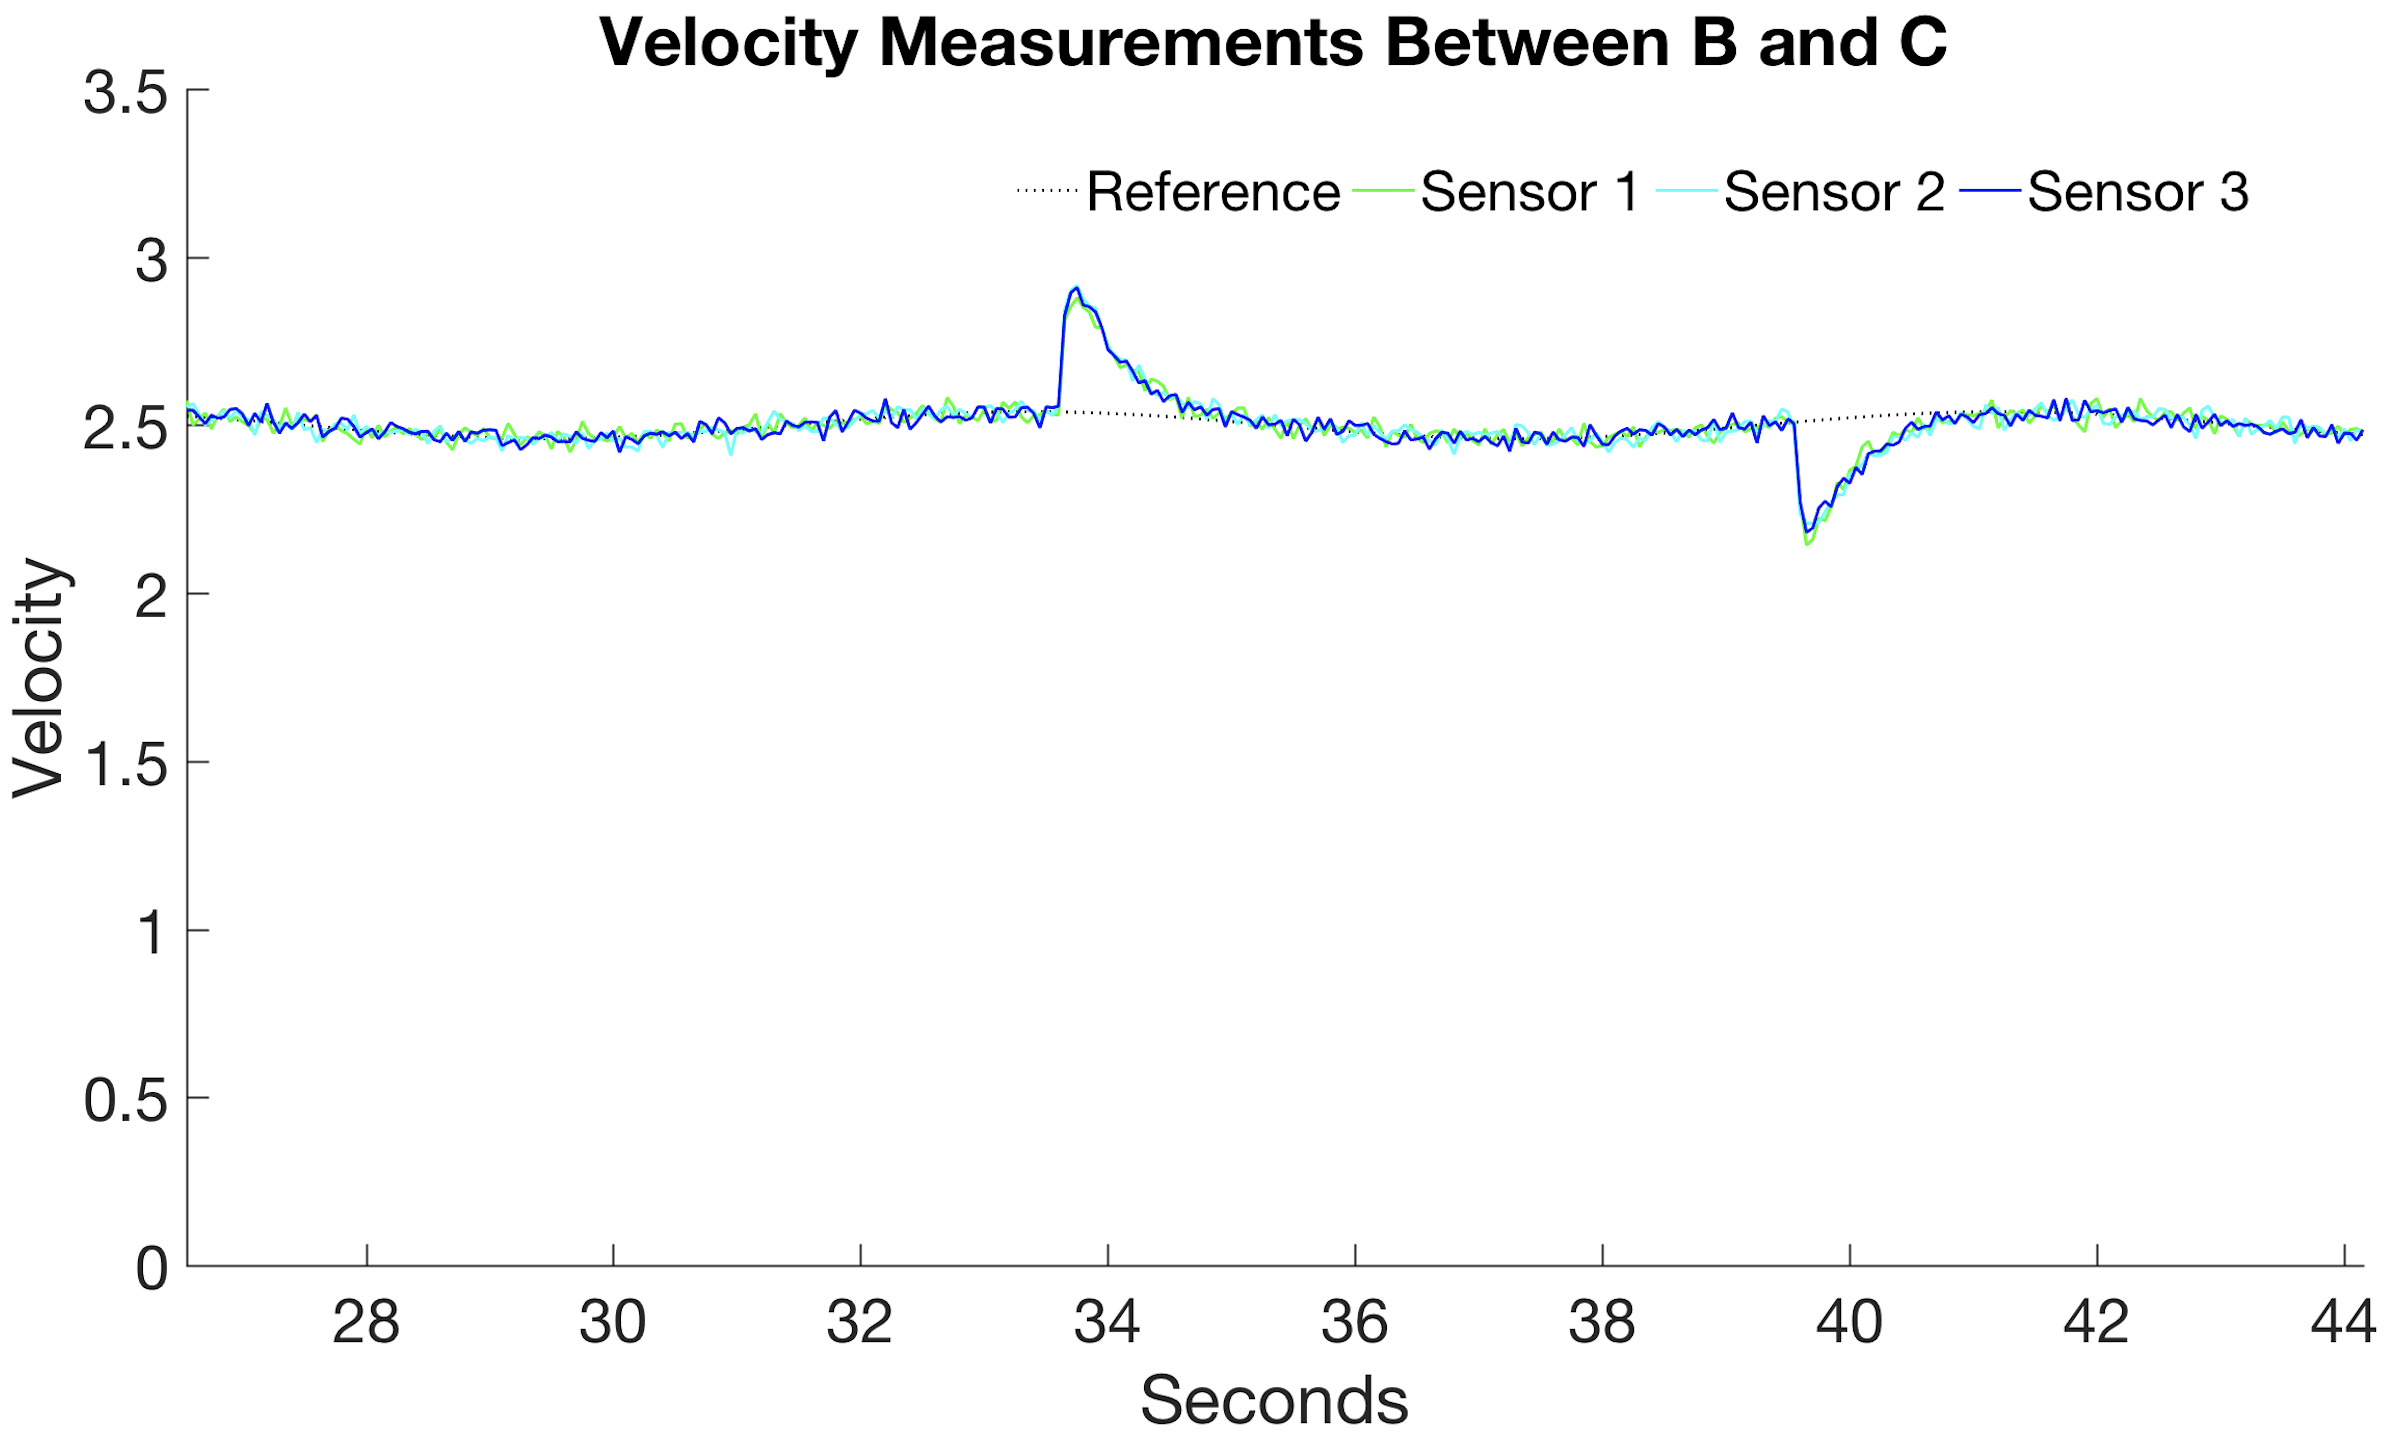
\includegraphics[width = 0.22\textwidth]{Figures/vel_Goals1and2.png}} &	
\subfigure[\label{fig:input_G1and2} ]{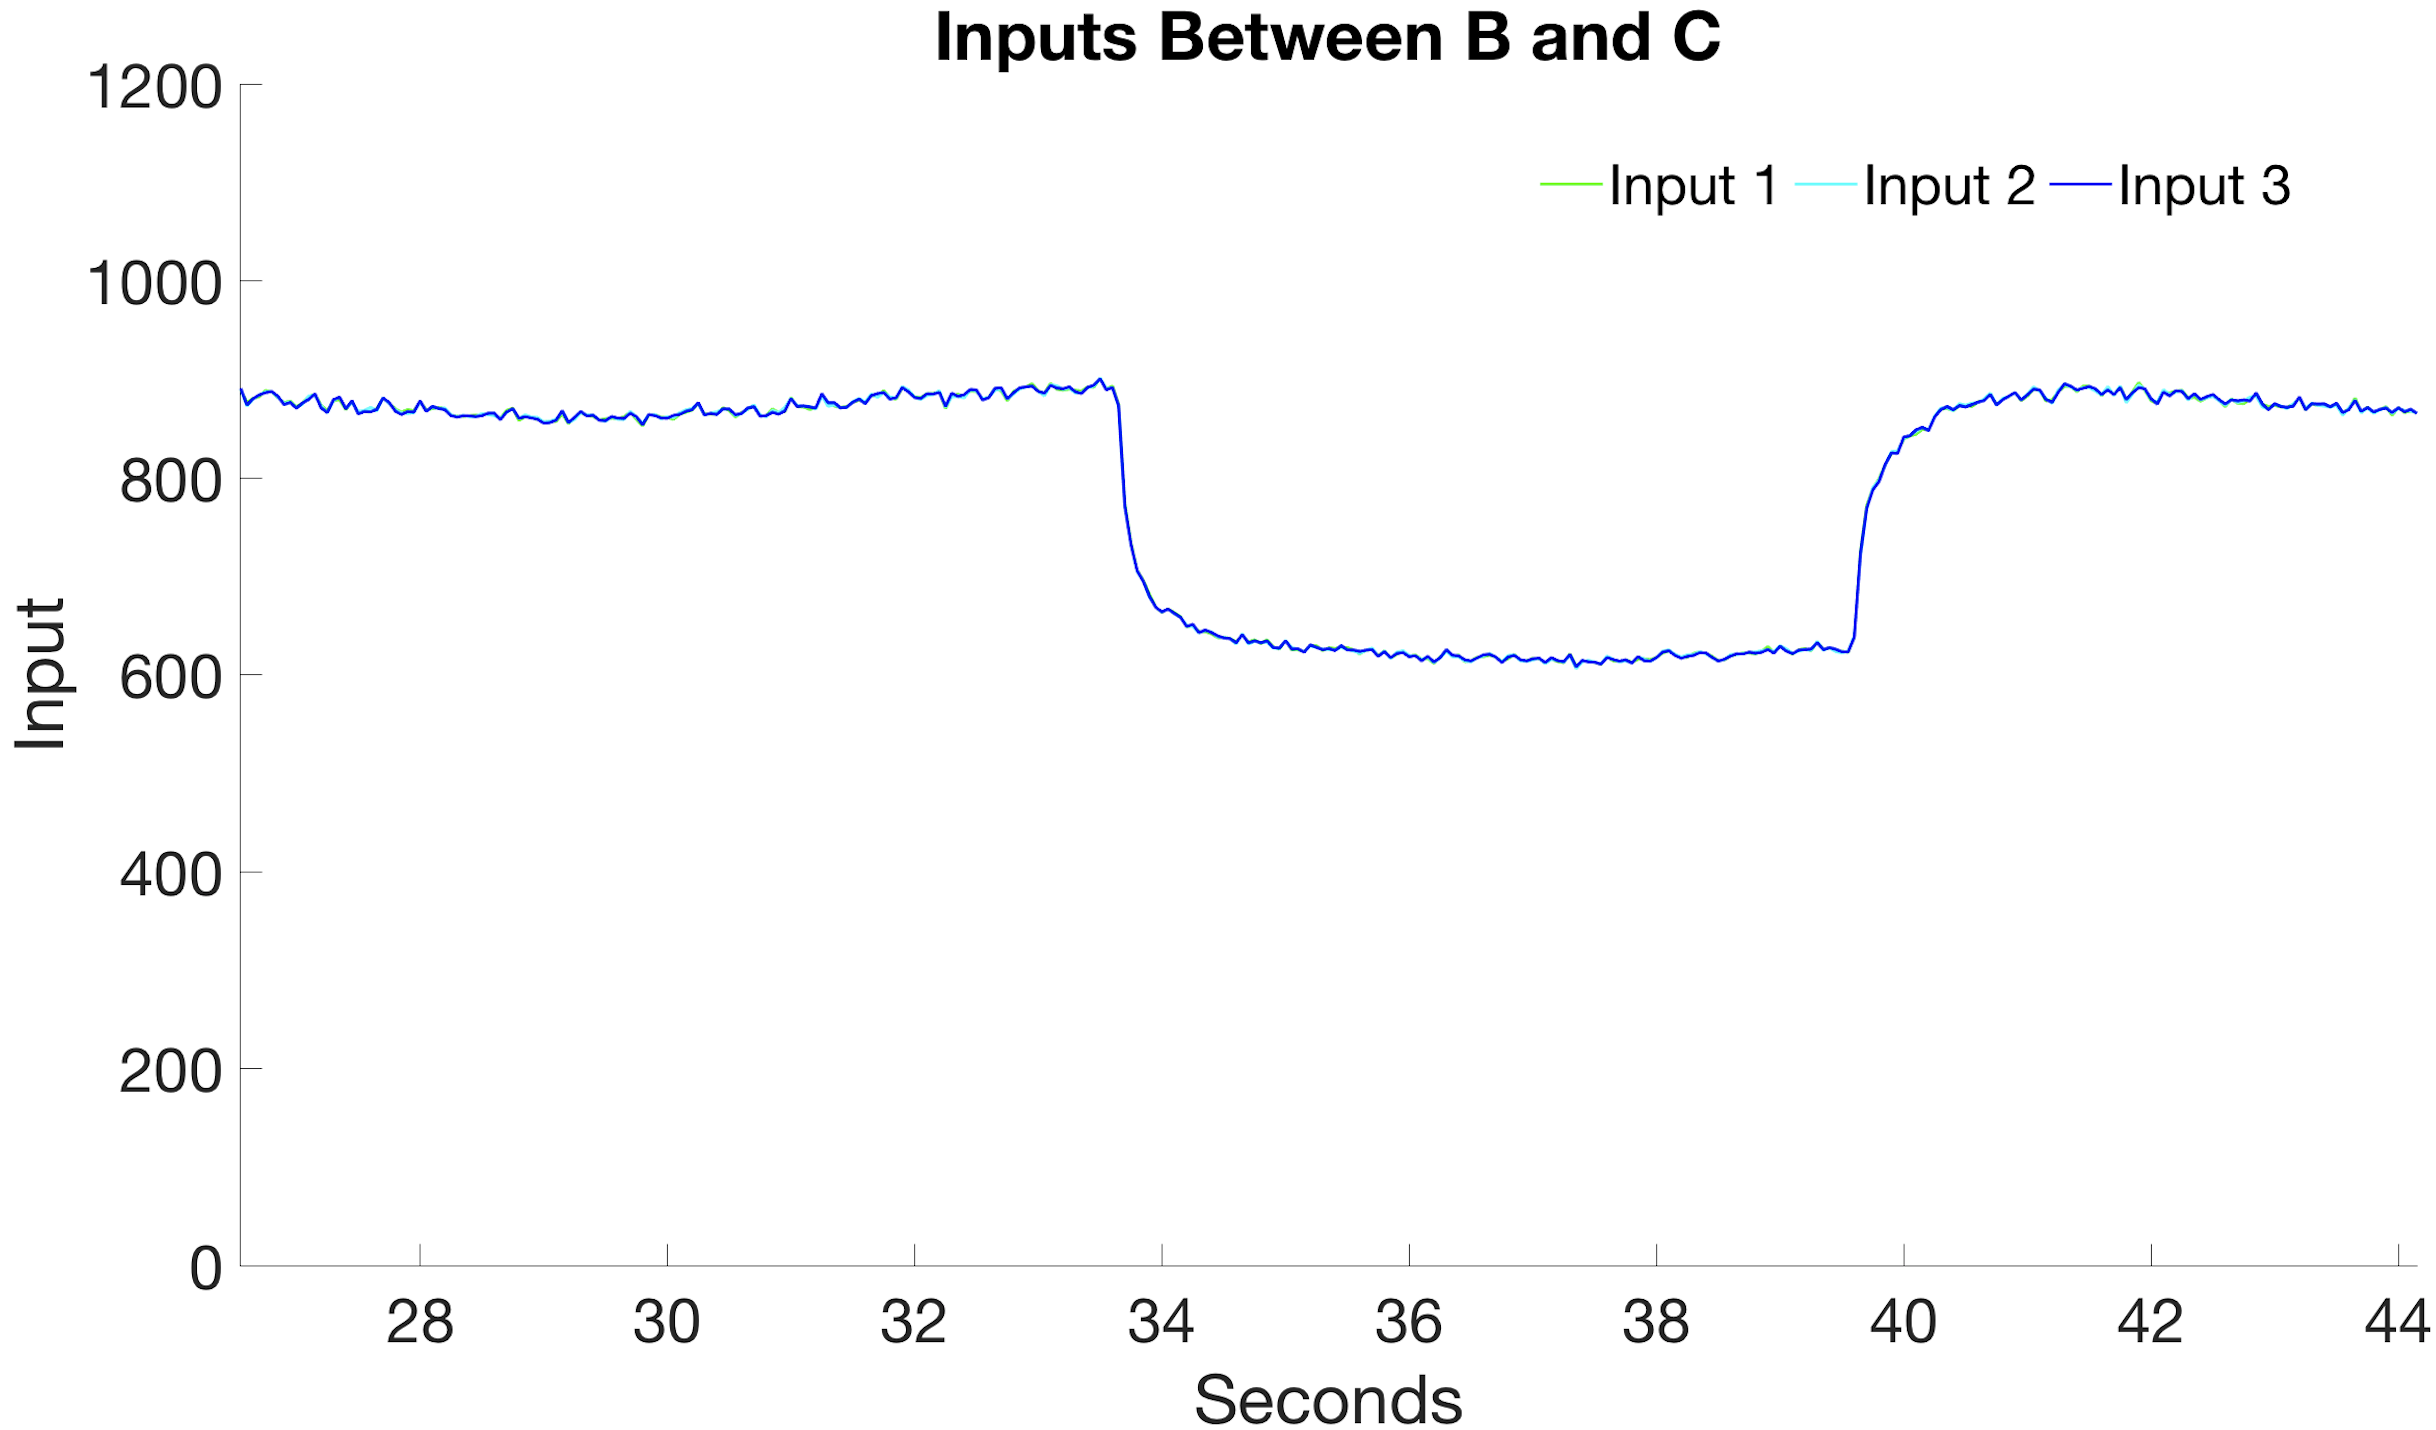
\includegraphics[width = 0.22\textwidth]{Figures/Inputs_Goals1and2.png}}

\end{tabular}
\label{fig:Goals1and2}
\caption{The vehicle is traveling between Goals 1 and 2 with all sensors uncompromised. System dynamics are changing between the goal points.}
\end{figure}



\begin{figure}
\vspace{1pt}
\centering
\begin{tabular}{cc}
\subfigure[\label{fig:vel_G2and3} ]{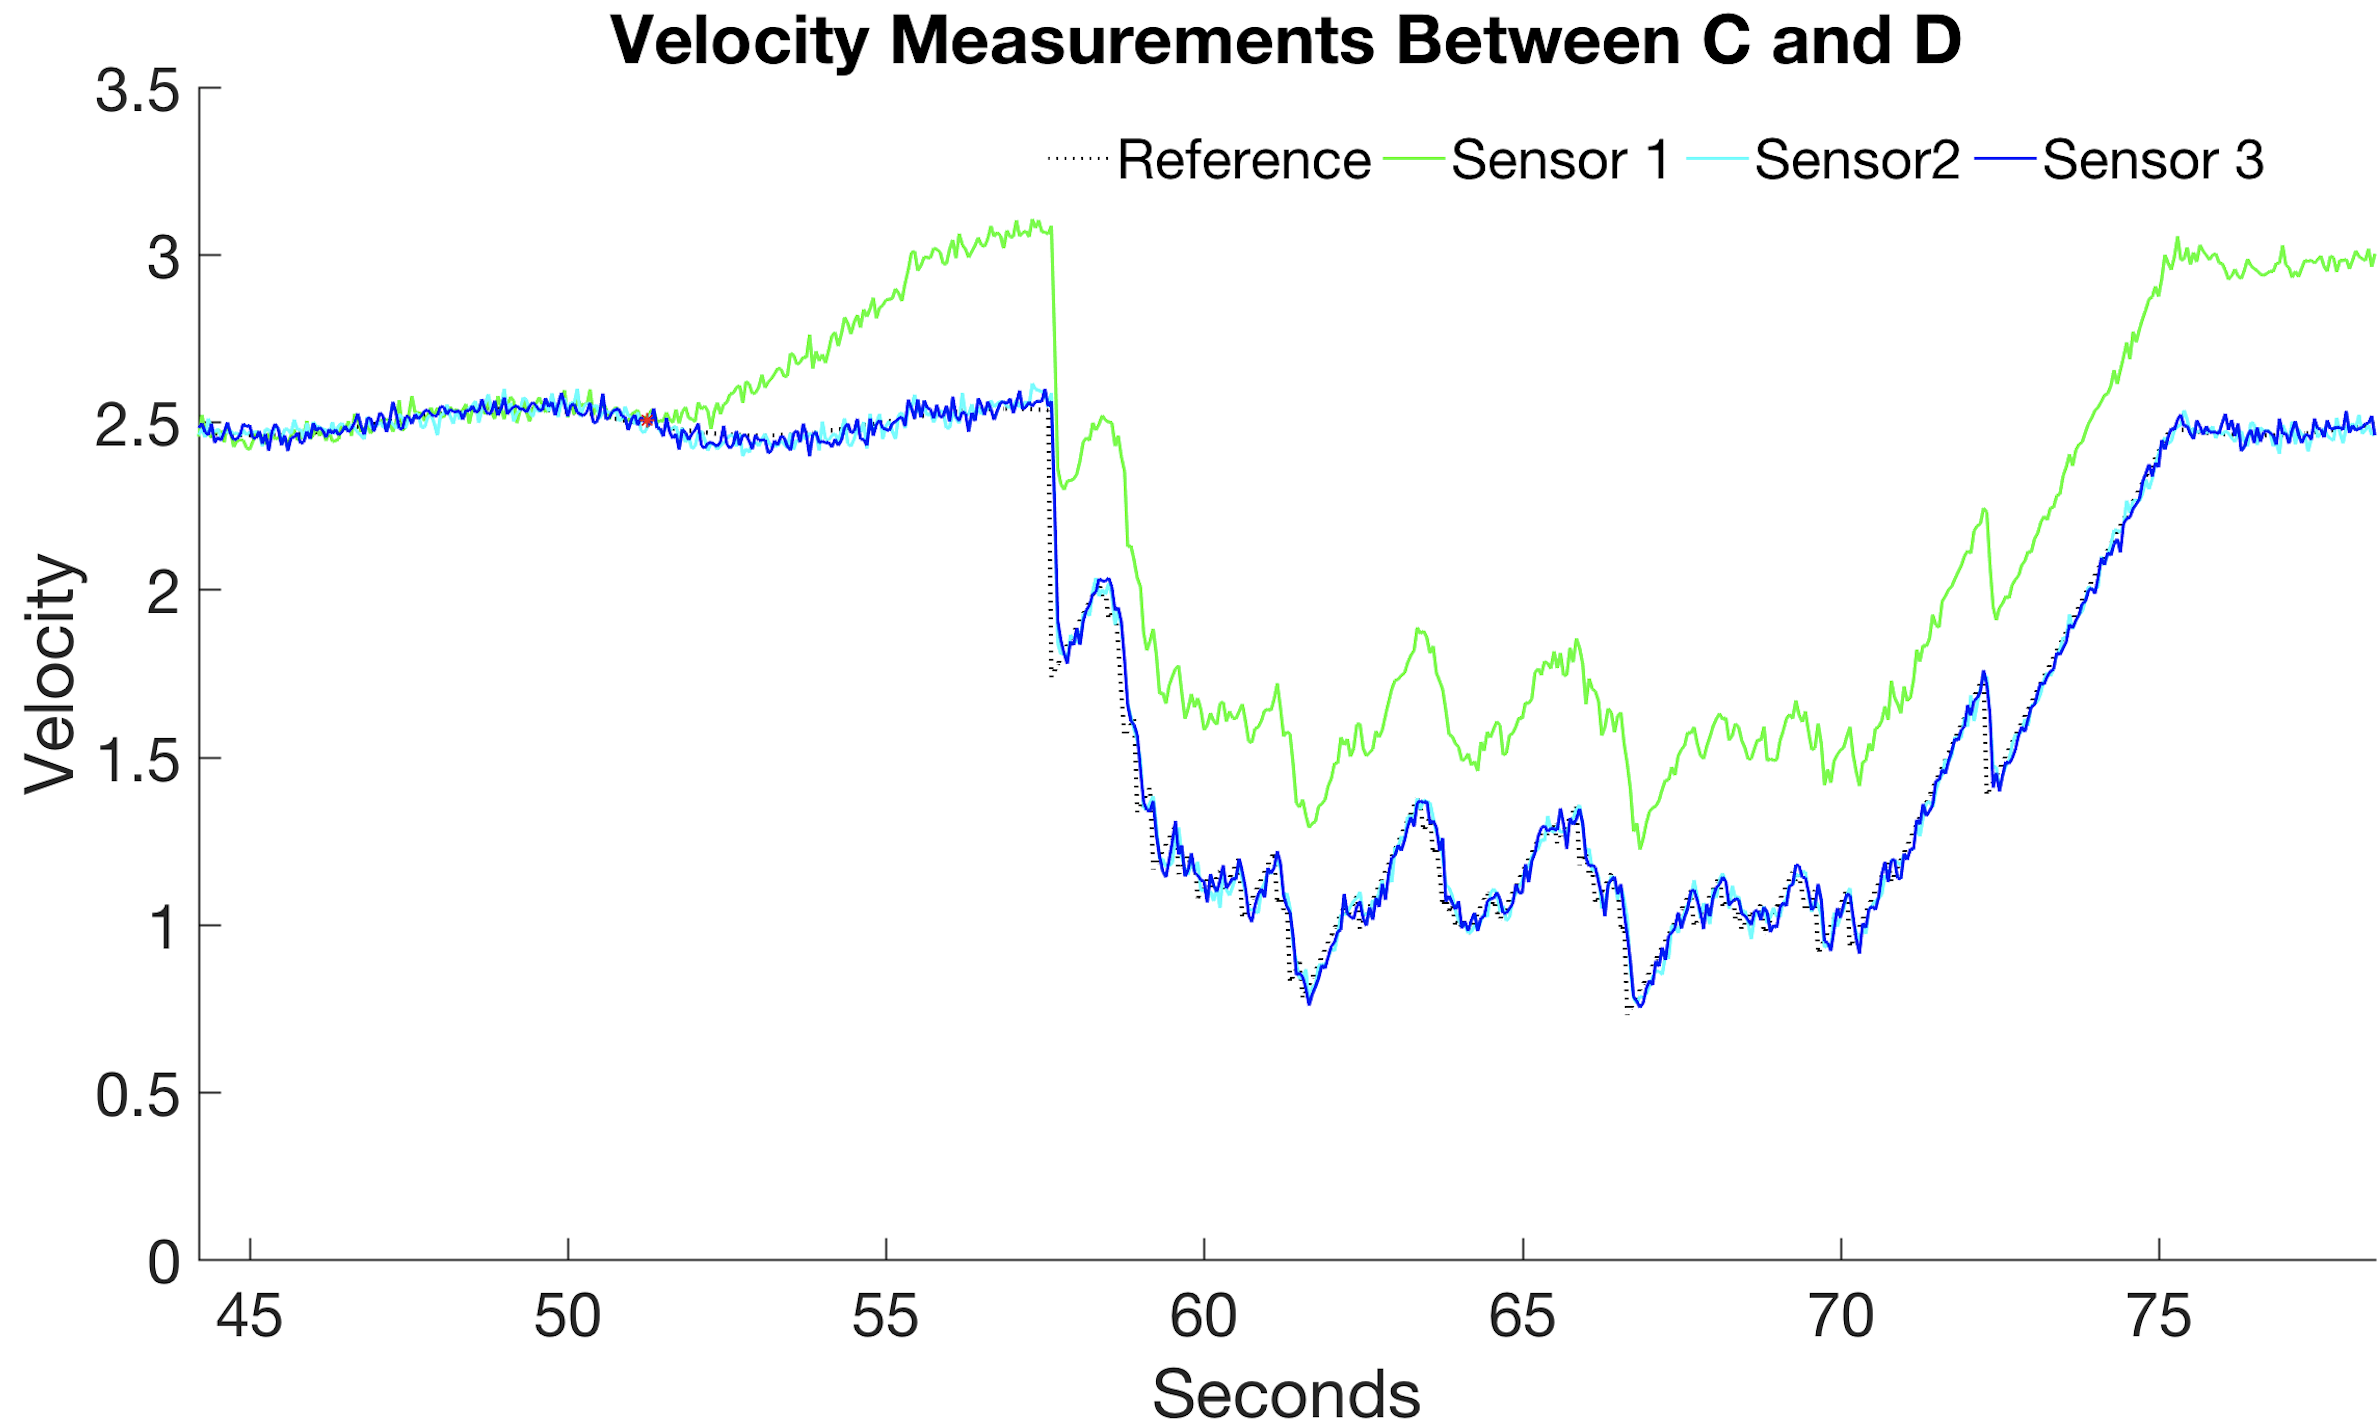
\includegraphics[width = 0.22\textwidth]{Figures/vel_Goals2and3.png}} & 
\subfigure[\label{fig:input_G2and3} ]{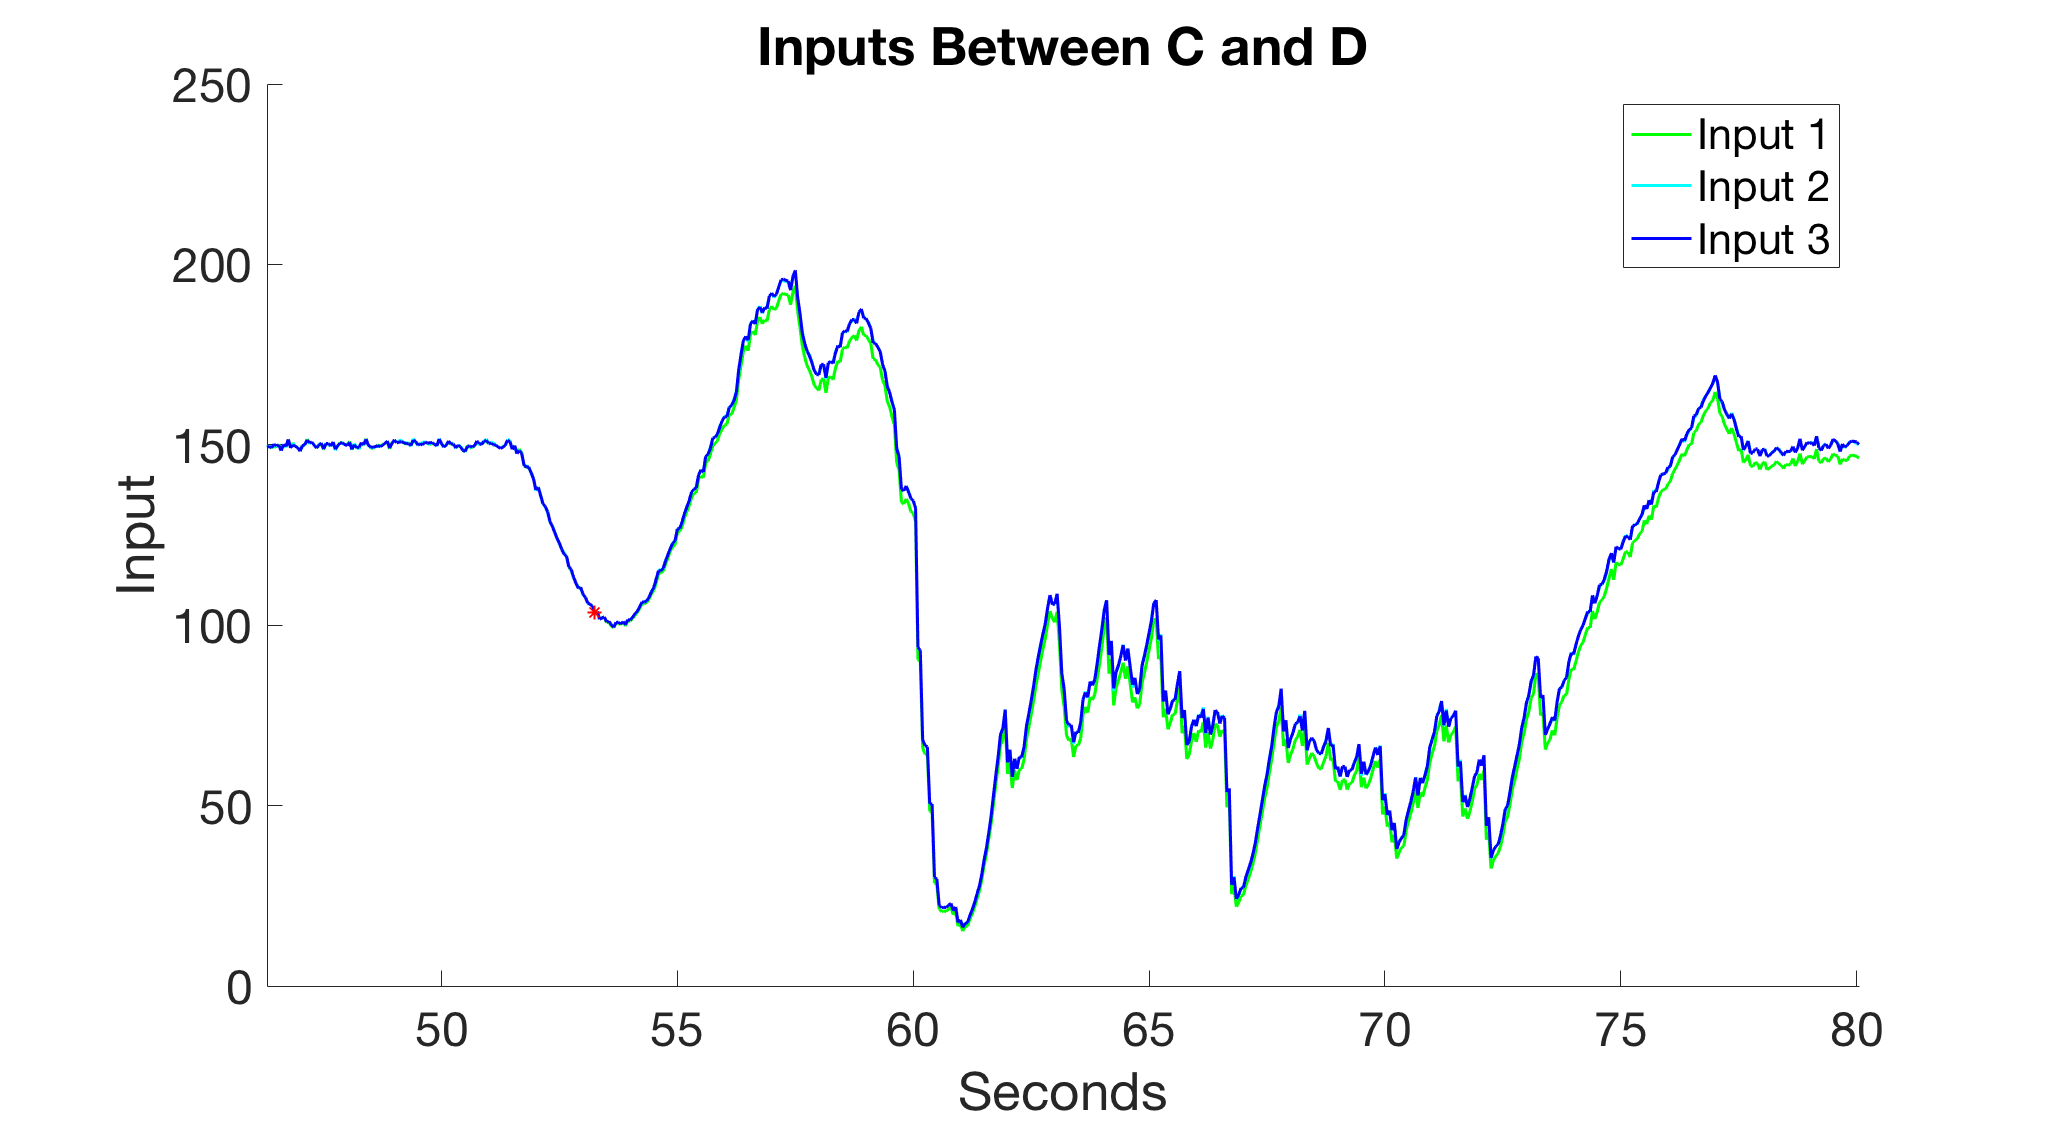
\includegraphics[width =0.22\textwidth]{Figures/Inputs_Goals2and3.png}}
\end{tabular}
\label{fig:Goals2and3}
\caption{The vehicle is traveling between Goals 2 and 3 where the vehicle encounters a sensor attack. Detection of this attack occurs, dropping the compromised sensor, allowing the vehicle to follow the desired velocity. With a higher uncertainty of the available sensor set, velocity is adapted to ensure vehicle safety . }
\end{figure}

\begin{figure}
\vspace{1pt}
\centering
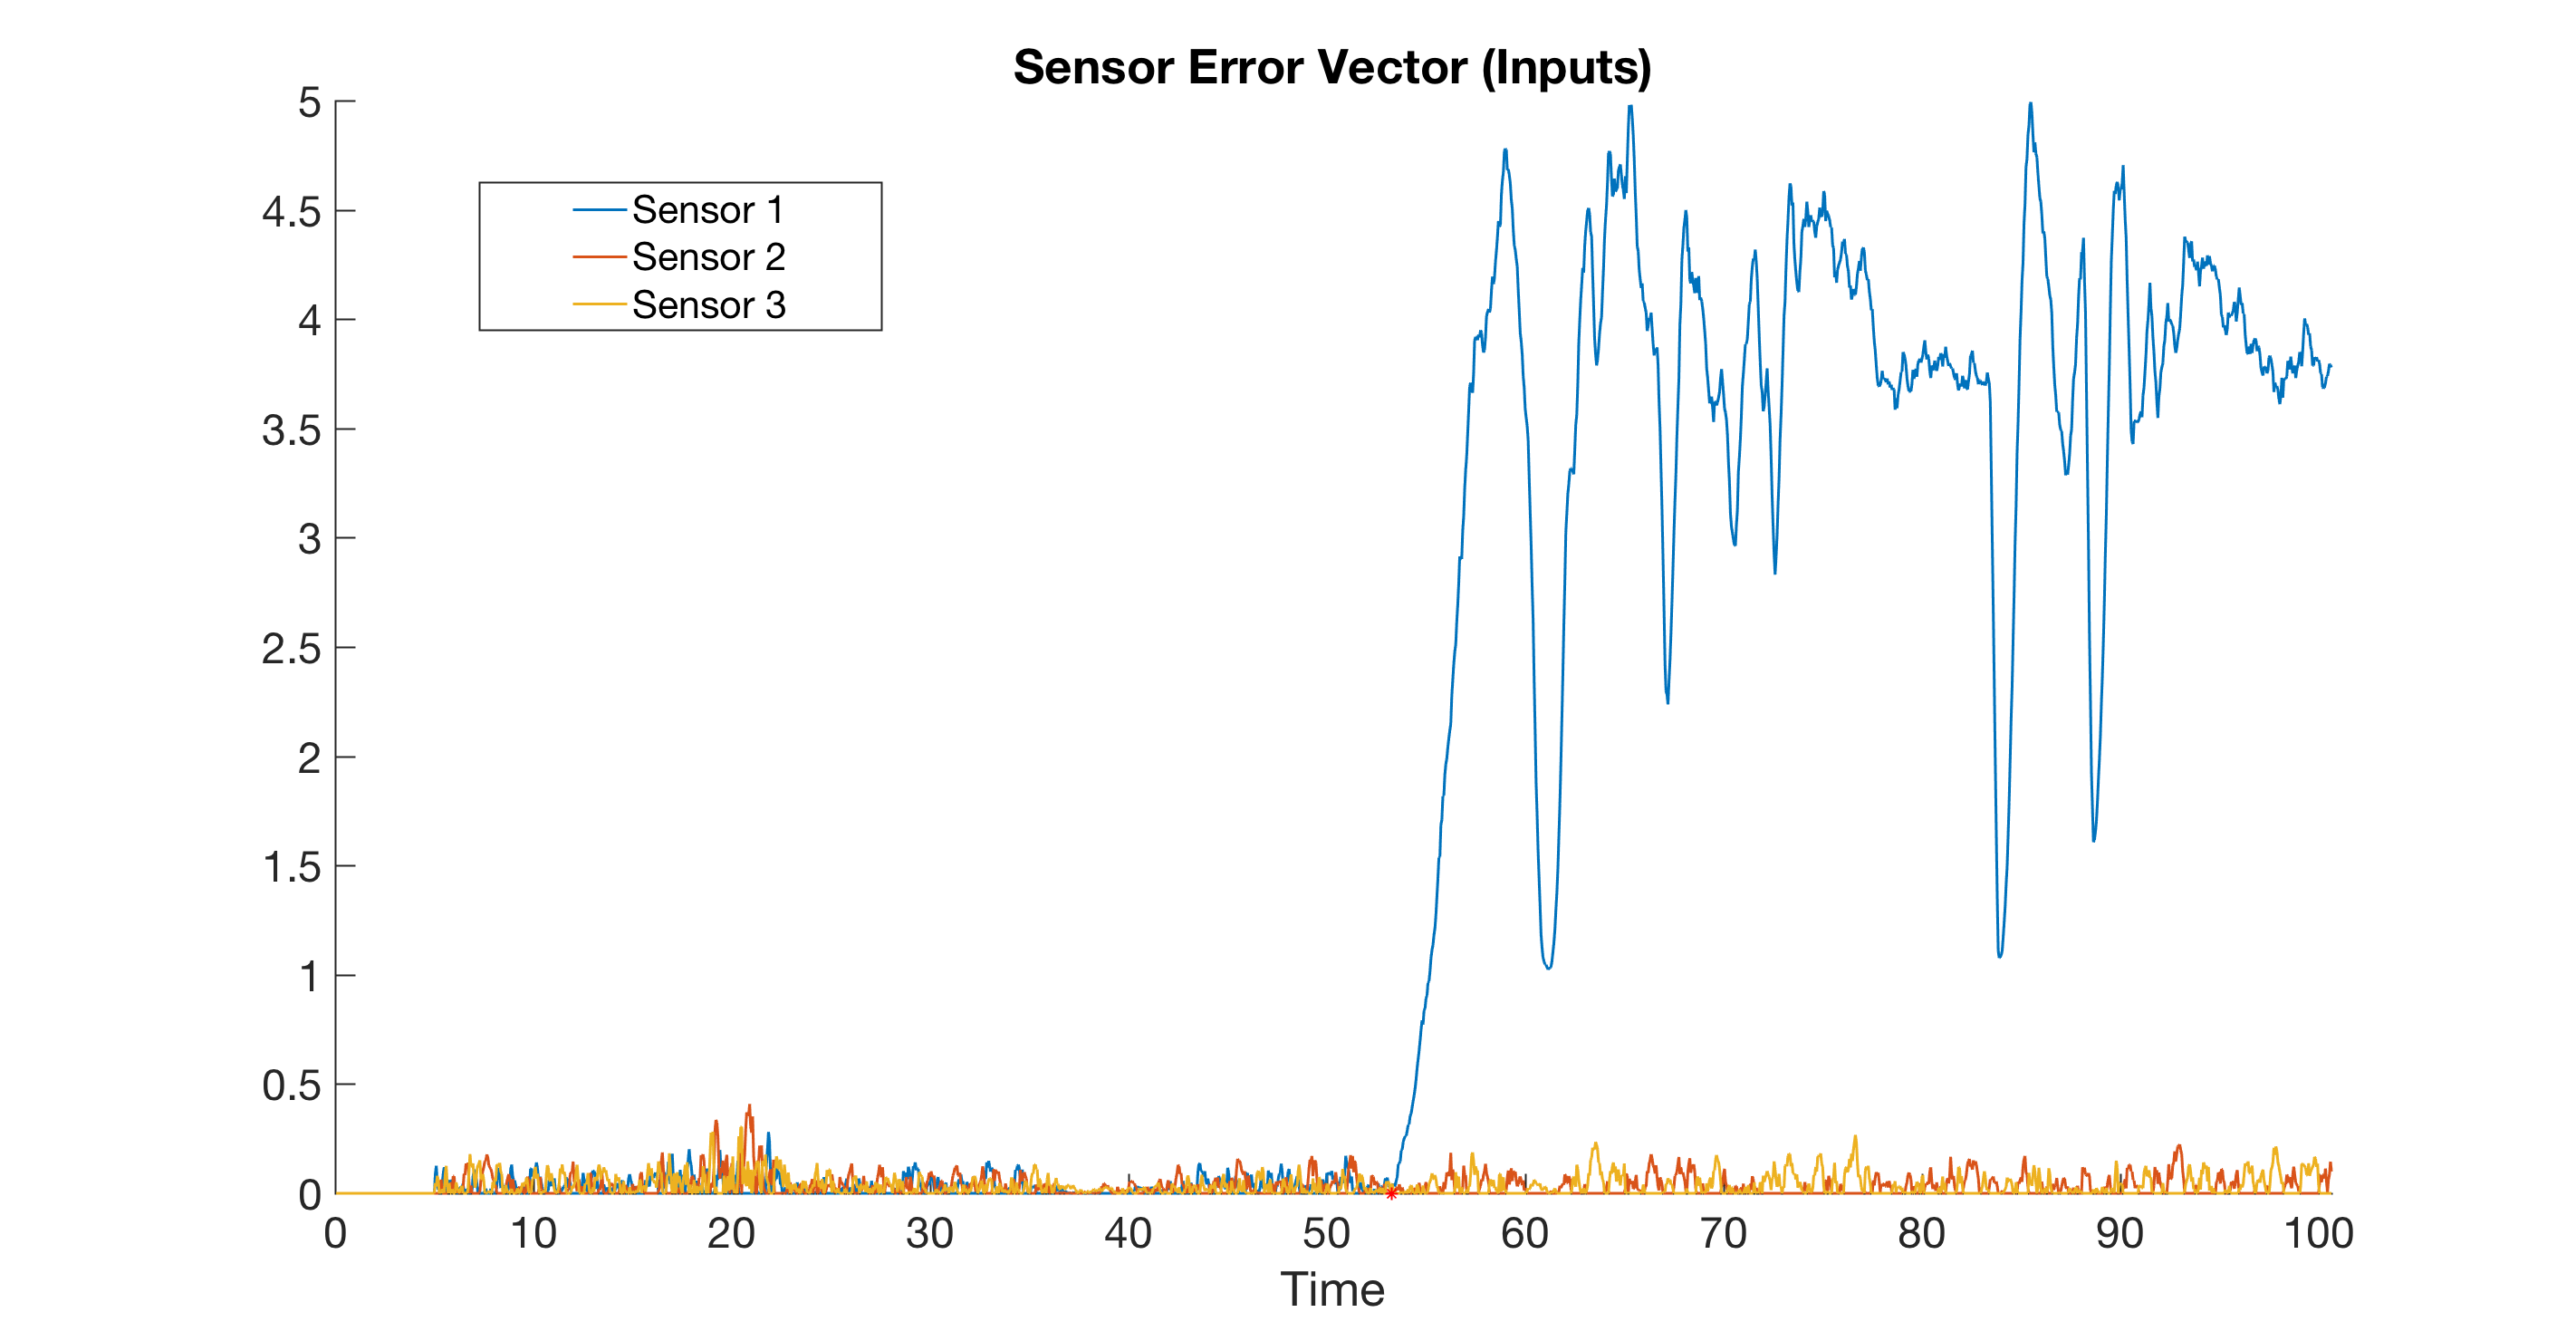
\includegraphics[width=0.48\textwidth]{Figures/Error_Vector.png}
\caption{The error vector is computing magnitudes of error for each of the sensors. As a sensor's error reaches a threshold, the sensor will be removed from the system.}
\label{fig:sensor error}
\end{figure}

\begin{figure}
\vspace{1pt}
\centering
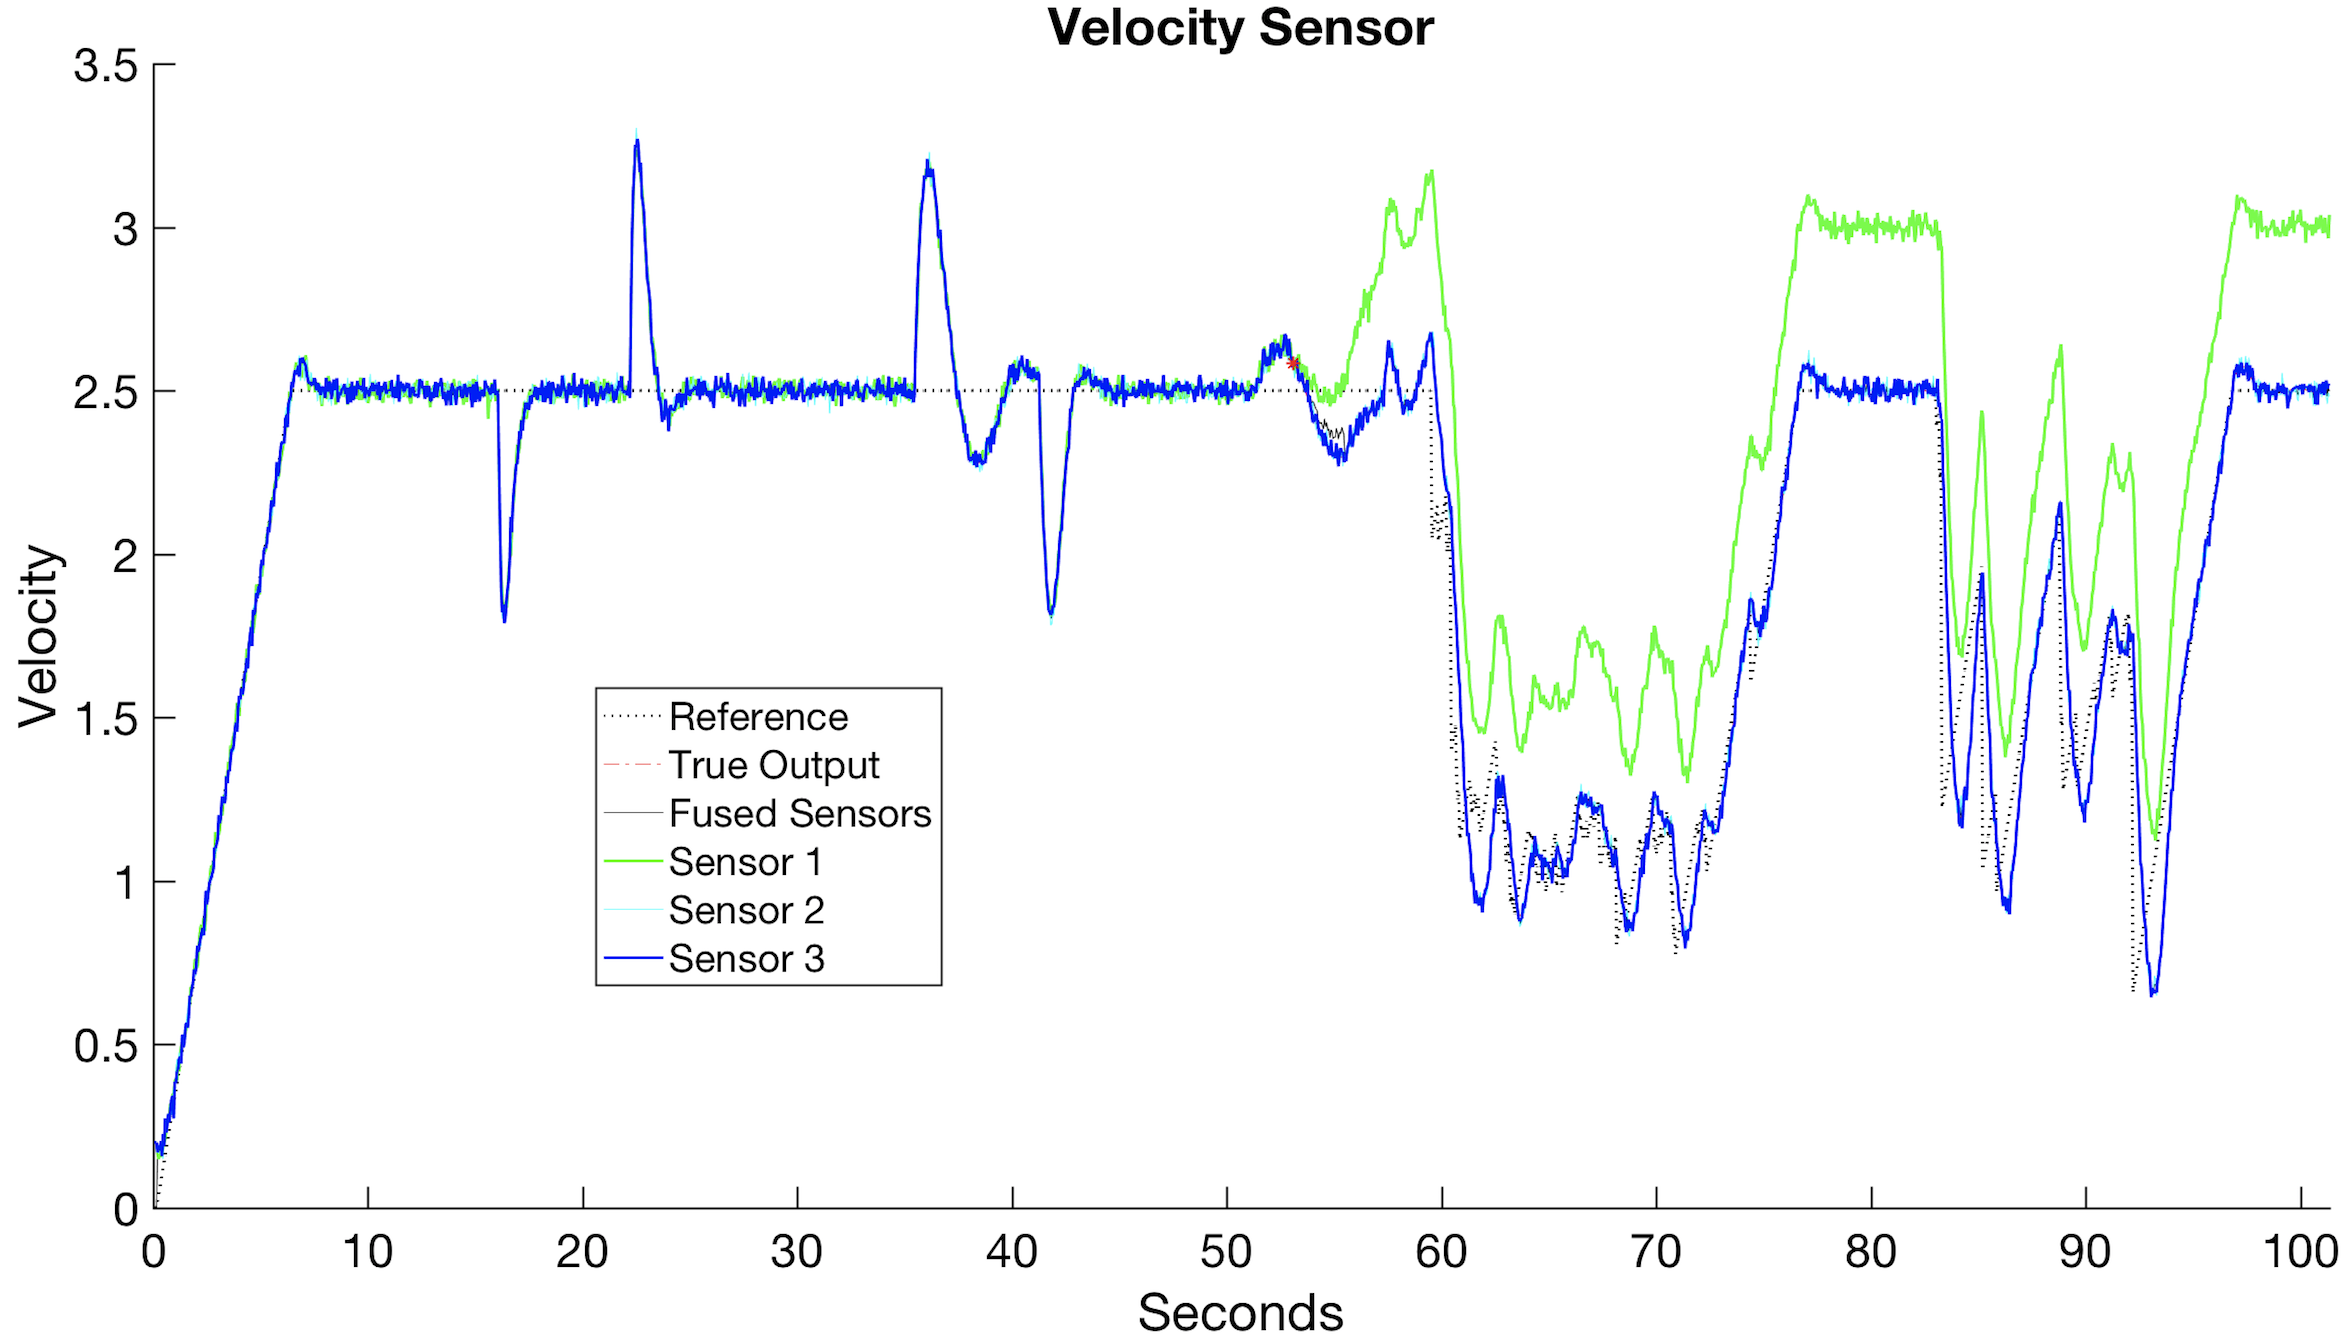
\includegraphics[width=0.48\textwidth]{Figures/Velocities.png}
\caption{Velocities are shown over the entire simulation. Sensor 3 measurements are no longer used by the system as soon as it diverges from the remaining sensors. }
\label{fig:total_velocity}
\end{figure}

% \begin{figure}
% \vspace{1pt}
% \centering
% 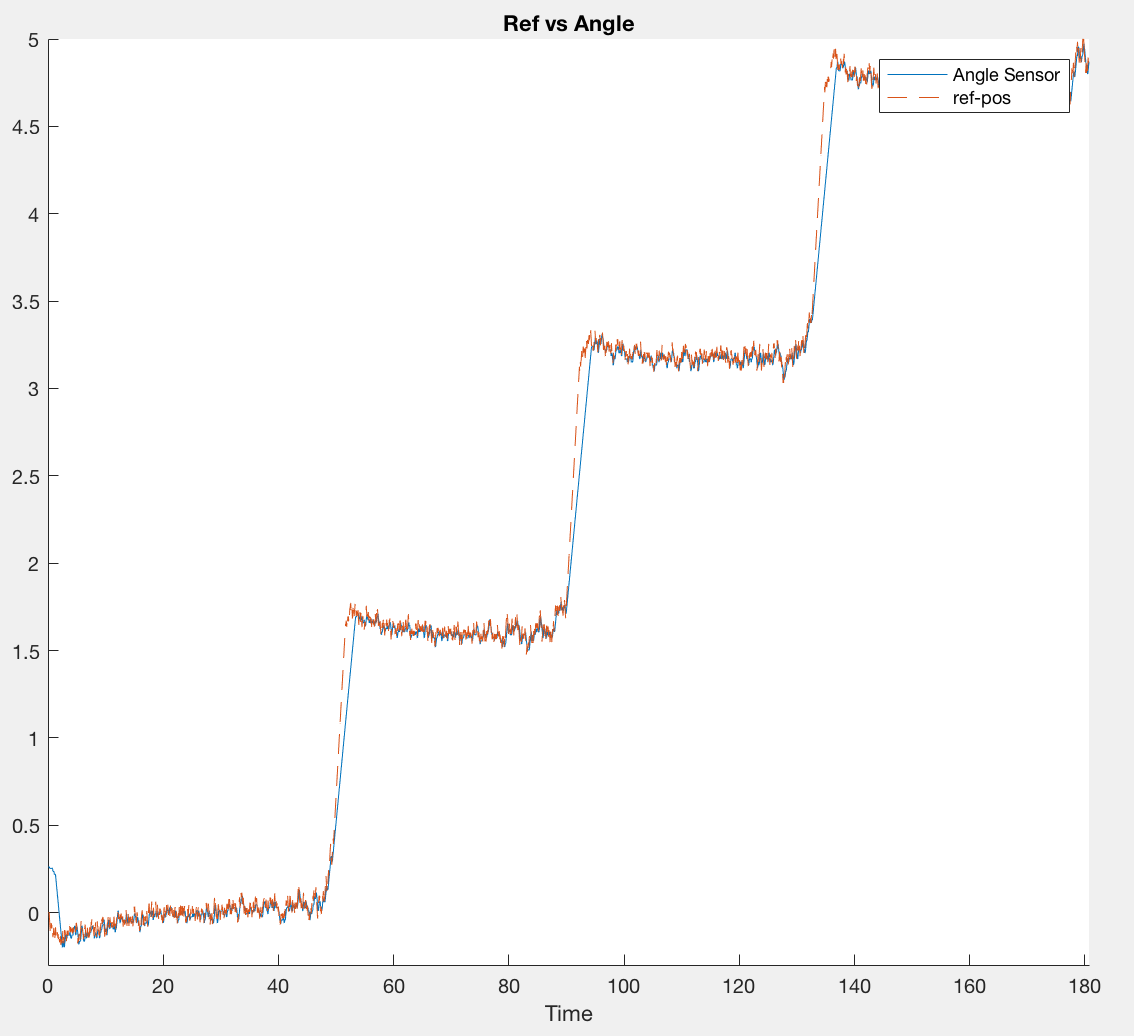
\includegraphics[width=0.48\textwidth]{ang_t.png}
% \caption{Vehicle heading angle over time exhibiting an attack on an angle sensor while the system detects and corrects.}
% \label{fig:ang_t}
% \end{figure}




\end{section}